%!TEX root = ../dissertation.tex
\begin{savequote}[75mm]
No person was ever honored for what he received. Honor has been the reward for what he gave.   
\end{savequote}
\chapter{Discussion on systematic uncertainties}
\label{app:appendixSys}

%%%%%%%%%%%%%%%%%%%%%%%%%%%%%%%%%%%%%%%%%%%%%%%%%%%%%%%%%%%%%%%%%%%%%%%
%%%%%%%%%%%%%%%%%%%%%%%%%%%%%%%%%%%%%%%%%%%%%%%%%%%%%%%%%%%%%%%%%%%%%%%
\section{Uncertainty on \ttbar~ generator}
\label{sec:ttbar-mc-unc}

\paragraph{}
In addition to the \ttbar~ fit uncertainties, additional \ttbar~ MC samples are considered with the following variations: hadronization (Had), fragmentation (Frag), additional radiation (Rad), and top quark mass (Mass).
The variation in total background, with different \ttbar~ MC samples as input is tested.
These \ttbar~ simulations are used to replace the nominal \ttbar~ MC and are stitched with the high $m_{t\bar{t}}$ samples. 
The variations in the $2bs$ signal region prediction are shown in Figure~\ref{fig:ttbar-MC}. 
This uncertainty is considered to be limited by the MC statistical uncertainties, and therefore no \ttbar~ MC uncertainty is applied.

\begin{figure}[htb!]
\begin{center} 
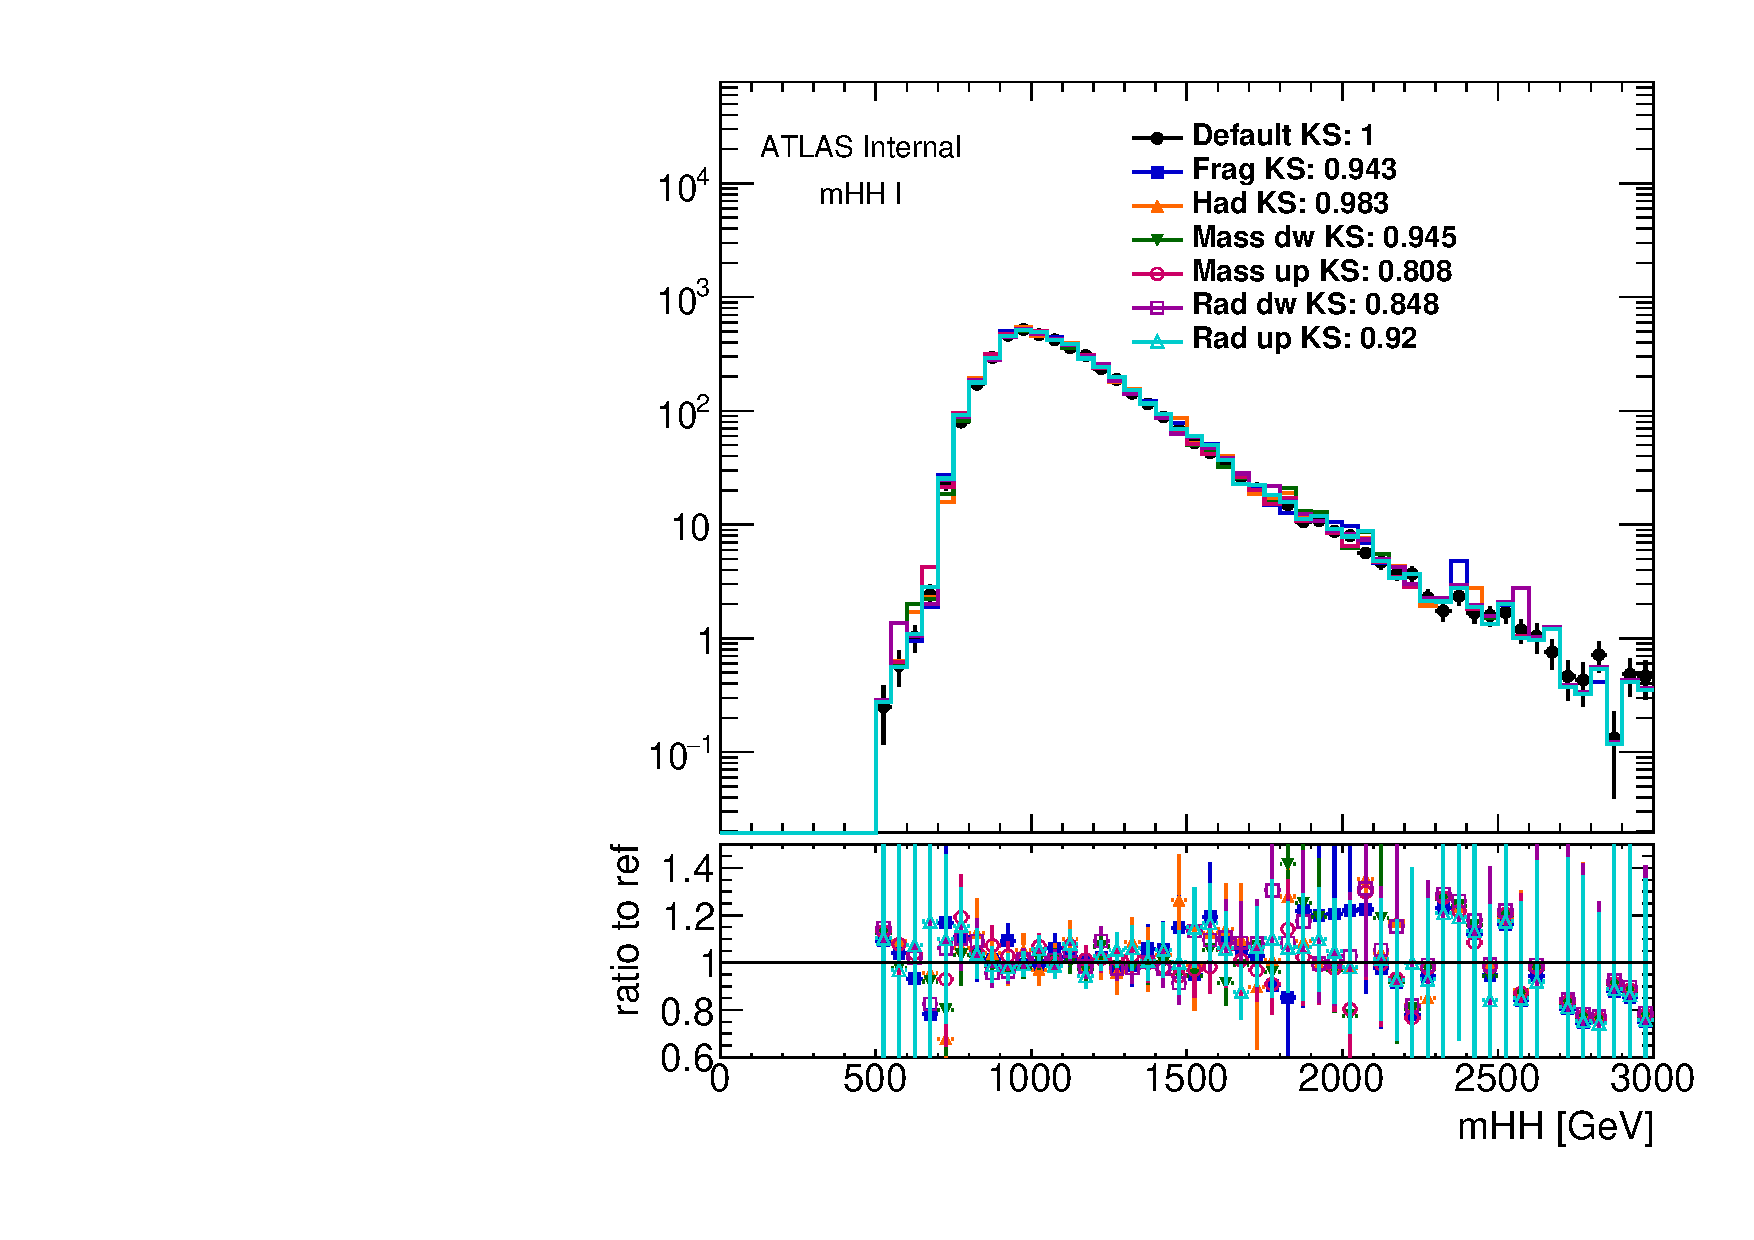
\includegraphics[width=0.48\textwidth,angle=-90]{figures/boosted/Other/directcompare_mHH_l_1_TwoTag_split_Top_syst_stat_postfit_all_.pdf}
\caption{$2bs$ channel signal region \mtwoJ~ total background (QCD + \ttbar) predictions with different \ttbar~ MC variations. The different variations agree with the nominal \ttbar~ MC within the statistical uncertainties.}
\label{fig:ttbar-MC}
\end{center}
\end{figure}

%%%%%%%%%%%%%%%%%%
\section{Uncertainty on the shape of \ttbar~ \mtwoJ~ in the $4/3b$ signal region}
\label{sec:unc-shape-ttbar-in-sr}

\paragraph{}
Because the \ttbar~ $4/3b$ sample is statistically limited, the $2bs$ \ttbar~ \mtwoJ~ shape is used to predict the \ttbar~ background shape in the $4/3b$ signal regions.
In order to estimate this shape uncertainty, the $2bs$ and $3b$ sideband shapes are normalized and compared in Figure~\ref{fig:ttbar-shapes-signal}.  
To avoid large statistical uncertainties, the distributions of the $3b$ and $2b$ are smoothed. 
The ratio of the two smoothed distributions is taken an additional \ttbar~ shape systematic. 
This ratio is used to scale the \ttbar~ background prediction in the signal region while keeping the same \ttbar~ yield.

\begin{figure}[htb!]
\begin{center} 
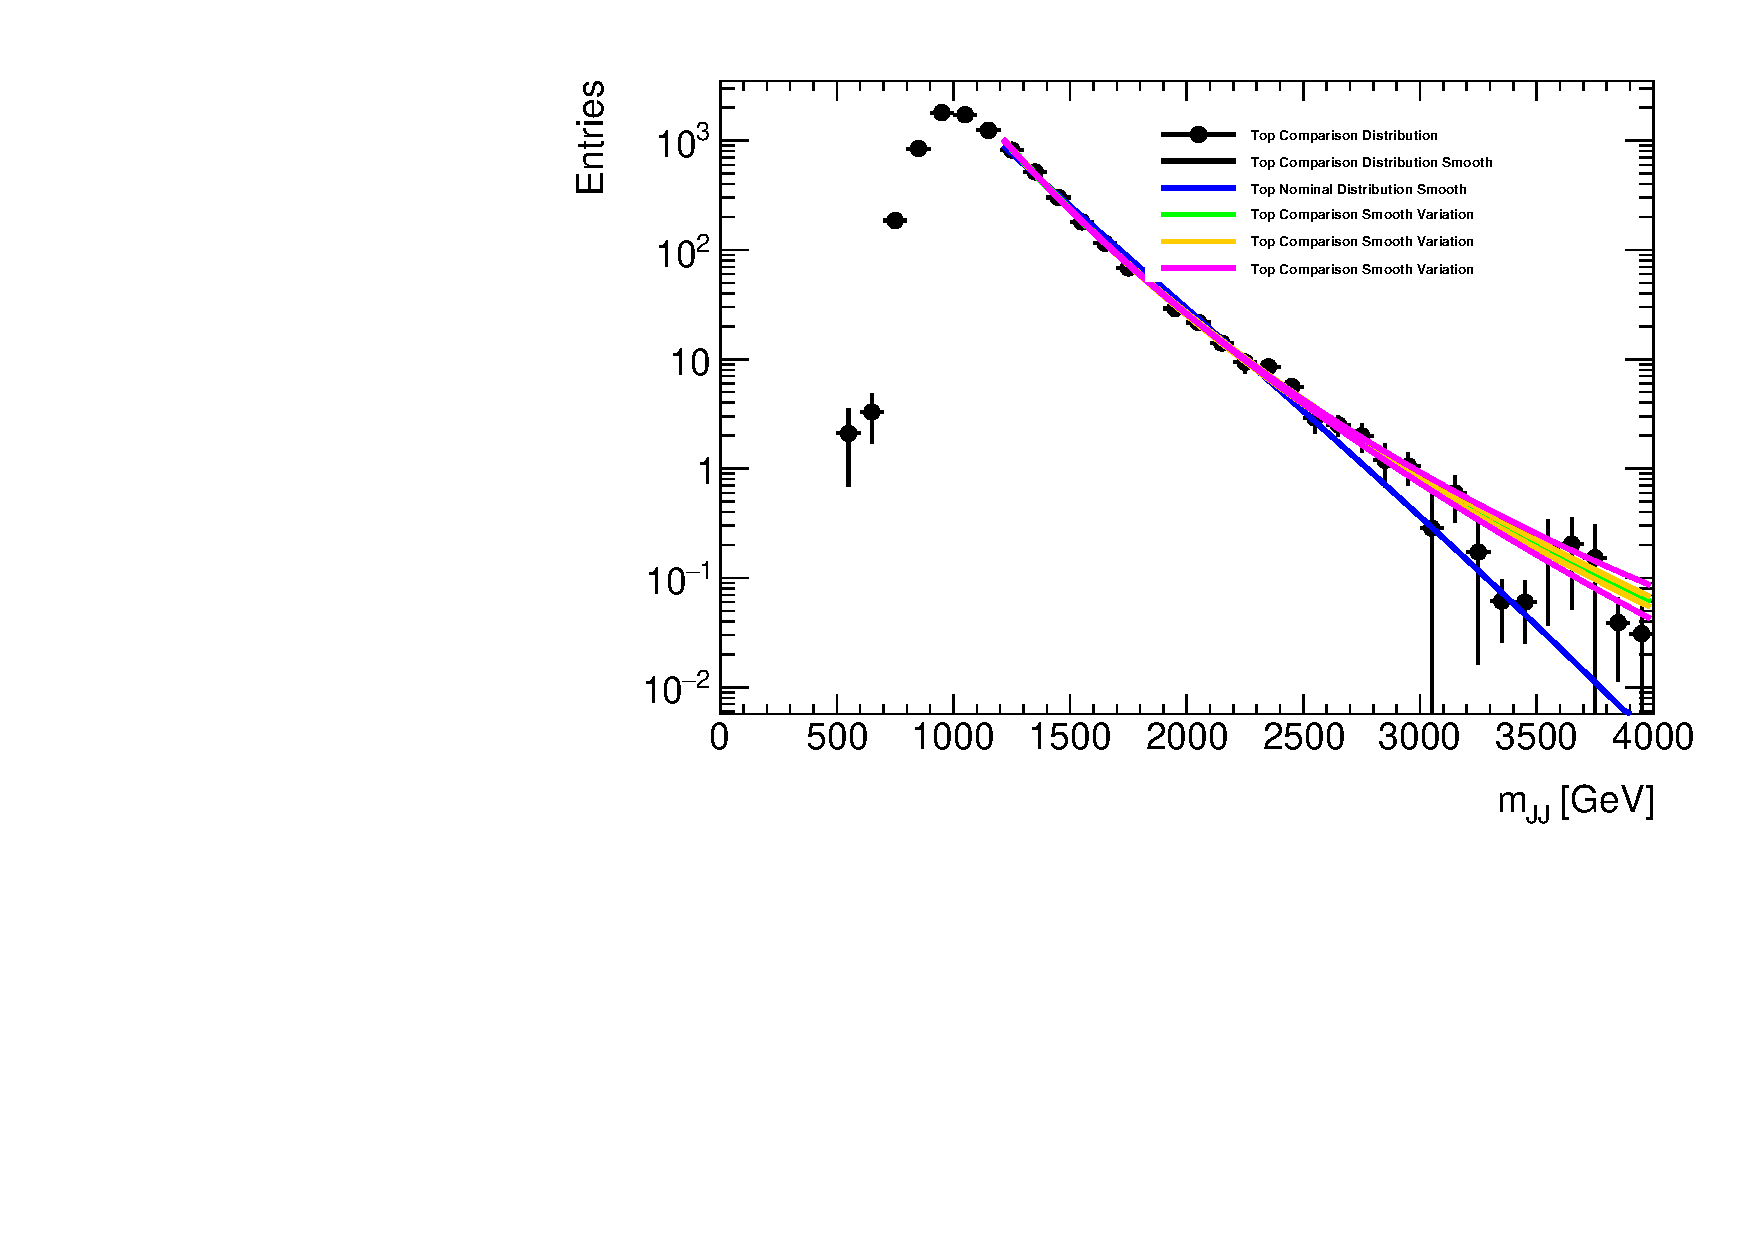
\includegraphics[width=0.31\textwidth,angle=-90]{figures/boosted/Syst_Smooth/TopShapeSRSysfitSmooth_sig33_comp22.pdf}
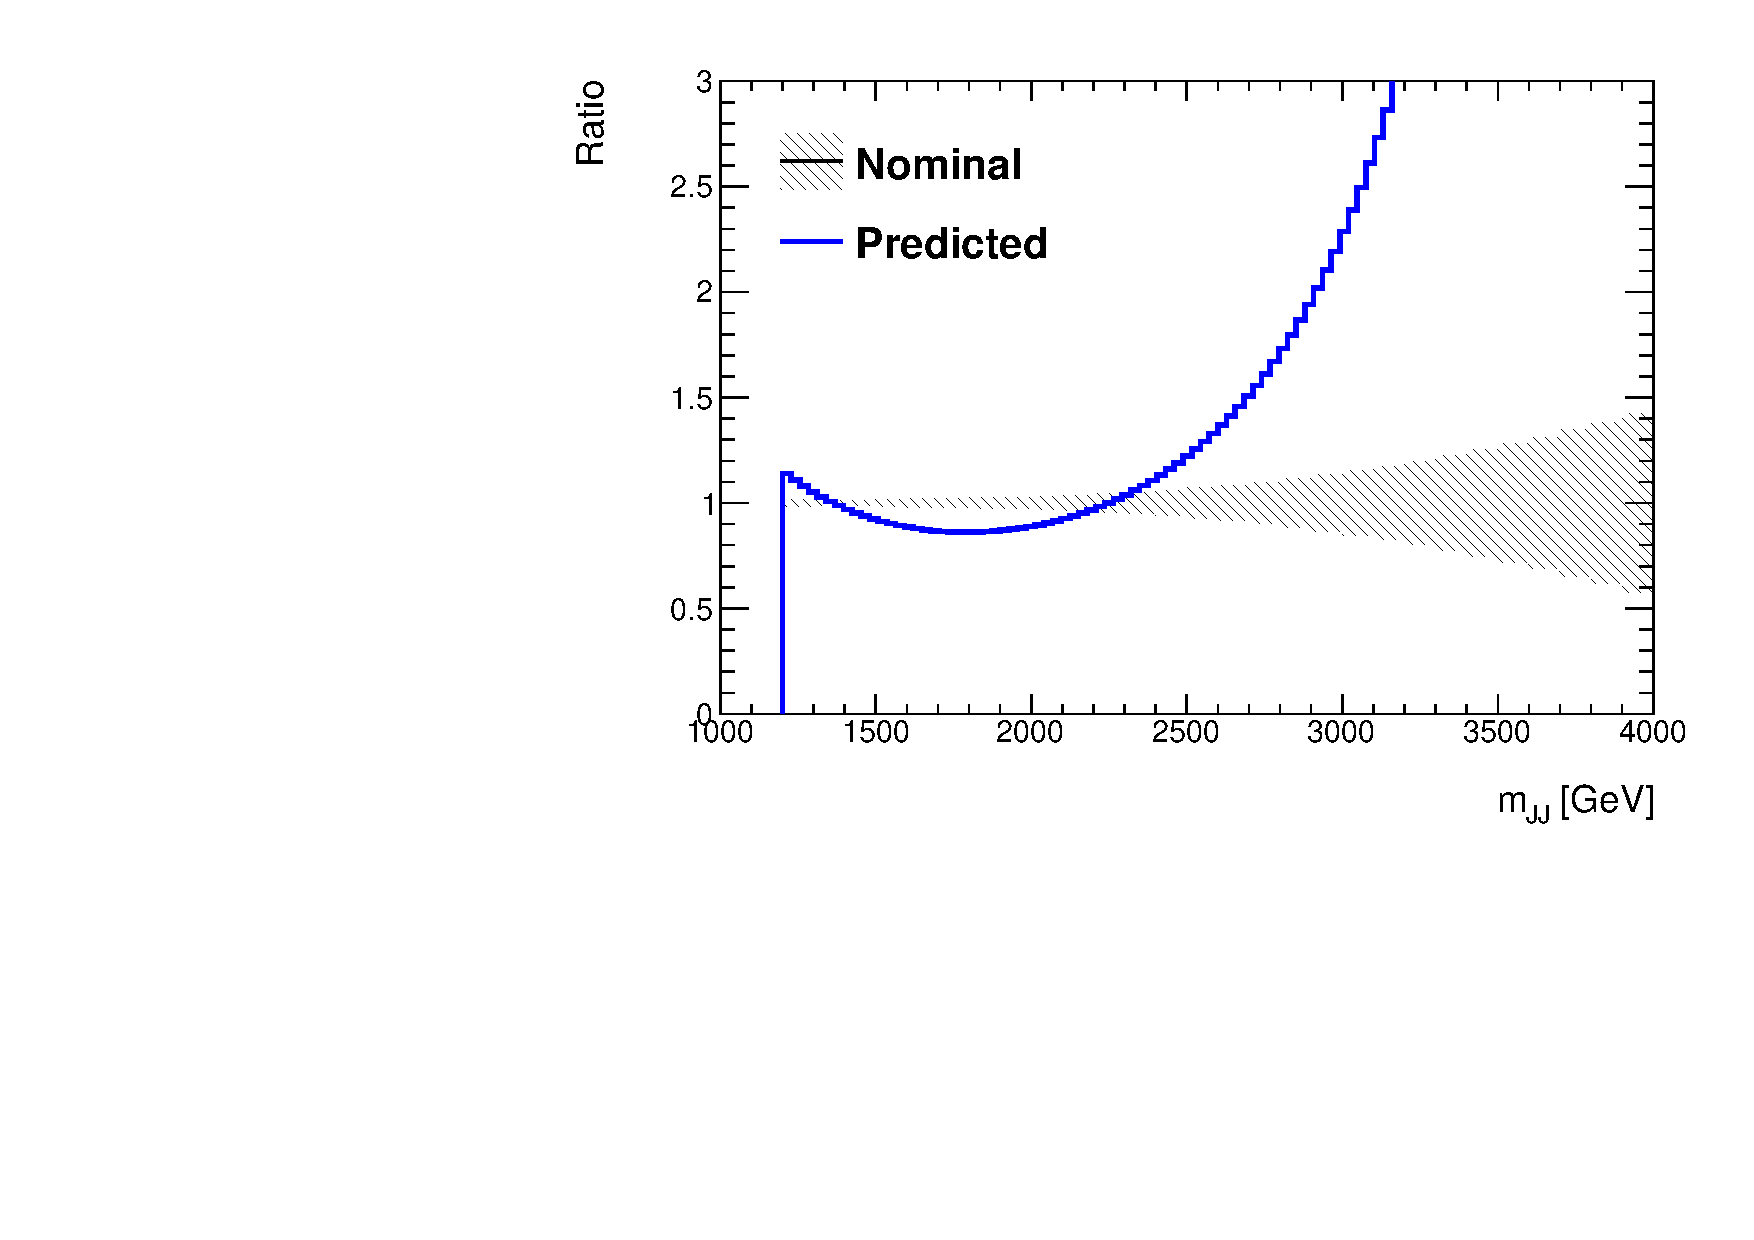
\includegraphics[width=0.31\textwidth,angle=-90]{figures/boosted/Syst_Smooth/TopShapeSRSysfitSmooth_sig33_comp22_ratio.pdf}
\caption{The shape of \ttbar~ \mtwoJ~ in the sideband region,
comparing the $3b$ shape with that of the $2bs$, in order to assess the systematic effect of additional $b$-tags changing the dijet mass distribution. The \mtwoJ~ distribution is shown on the left, and the ratio as a function of \mtwoJ~ between $3b$ and $2bs$ distributions is shown on the right.}
\label{fig:ttbar-shapes-signal}
\end{center}
\end{figure}

\section{Uncertainty on smoothing function in the signal region}
\label{unc-smooth-qcd-in-sr}

\paragraph{} 
While the function shown in Equation~\ref{eq:boosted_dijet} fits the predicted signal region \mtwoJ~ distribution well, it does not have a concrete, physical motivation.
Two checks are performed by varying the fit range and the fit function.
The checks show the smoothing function variations are almost always smaller than the statistical uncertainties of the distributions.
This gives this systematic uncertainty strong correlation with the shape uncertainties discussed in the previous section.
As a result, this systematic uncertainty is excluded.
Nevertheless, the tests are discussed below.

\paragraph{}
To test the impact of fit range, the upper bounds are varied to be $\{2800,\ 3000,\ 3200\}$ \GeV and the lower bounds are varied to be $\{1200,\ 1300,\ 1400\}$ \GeV.  
The ratio of the fits for each upper bound, to that of the nominal ($1200$-$3000$ \GeV) are shown in Figure~\ref{fig:qcd_fit_range_sys_ratio-scaled}, along with a hash band showing the statistical uncertainty of the nominal fit.
This is estimated separately for $2bs$, $3b$, and $4b$ samples.

\paragraph{}
Fits in which the fit $\chi^2$ per degree of freedom probability is less than $0.001\%$, or in which the fit integrals between $1500$-$2000$ \GeV, $2000$-$2500$ \GeV, or $>2500$ \GeV~ are not in agreement with the original distribution within a factor of $2$ or $0.5$, are not used to estimate the uncertainty. This ensure that poor fits are not used to estimate the uncertainty.

\begin{figure}[htb!]
\begin{center}
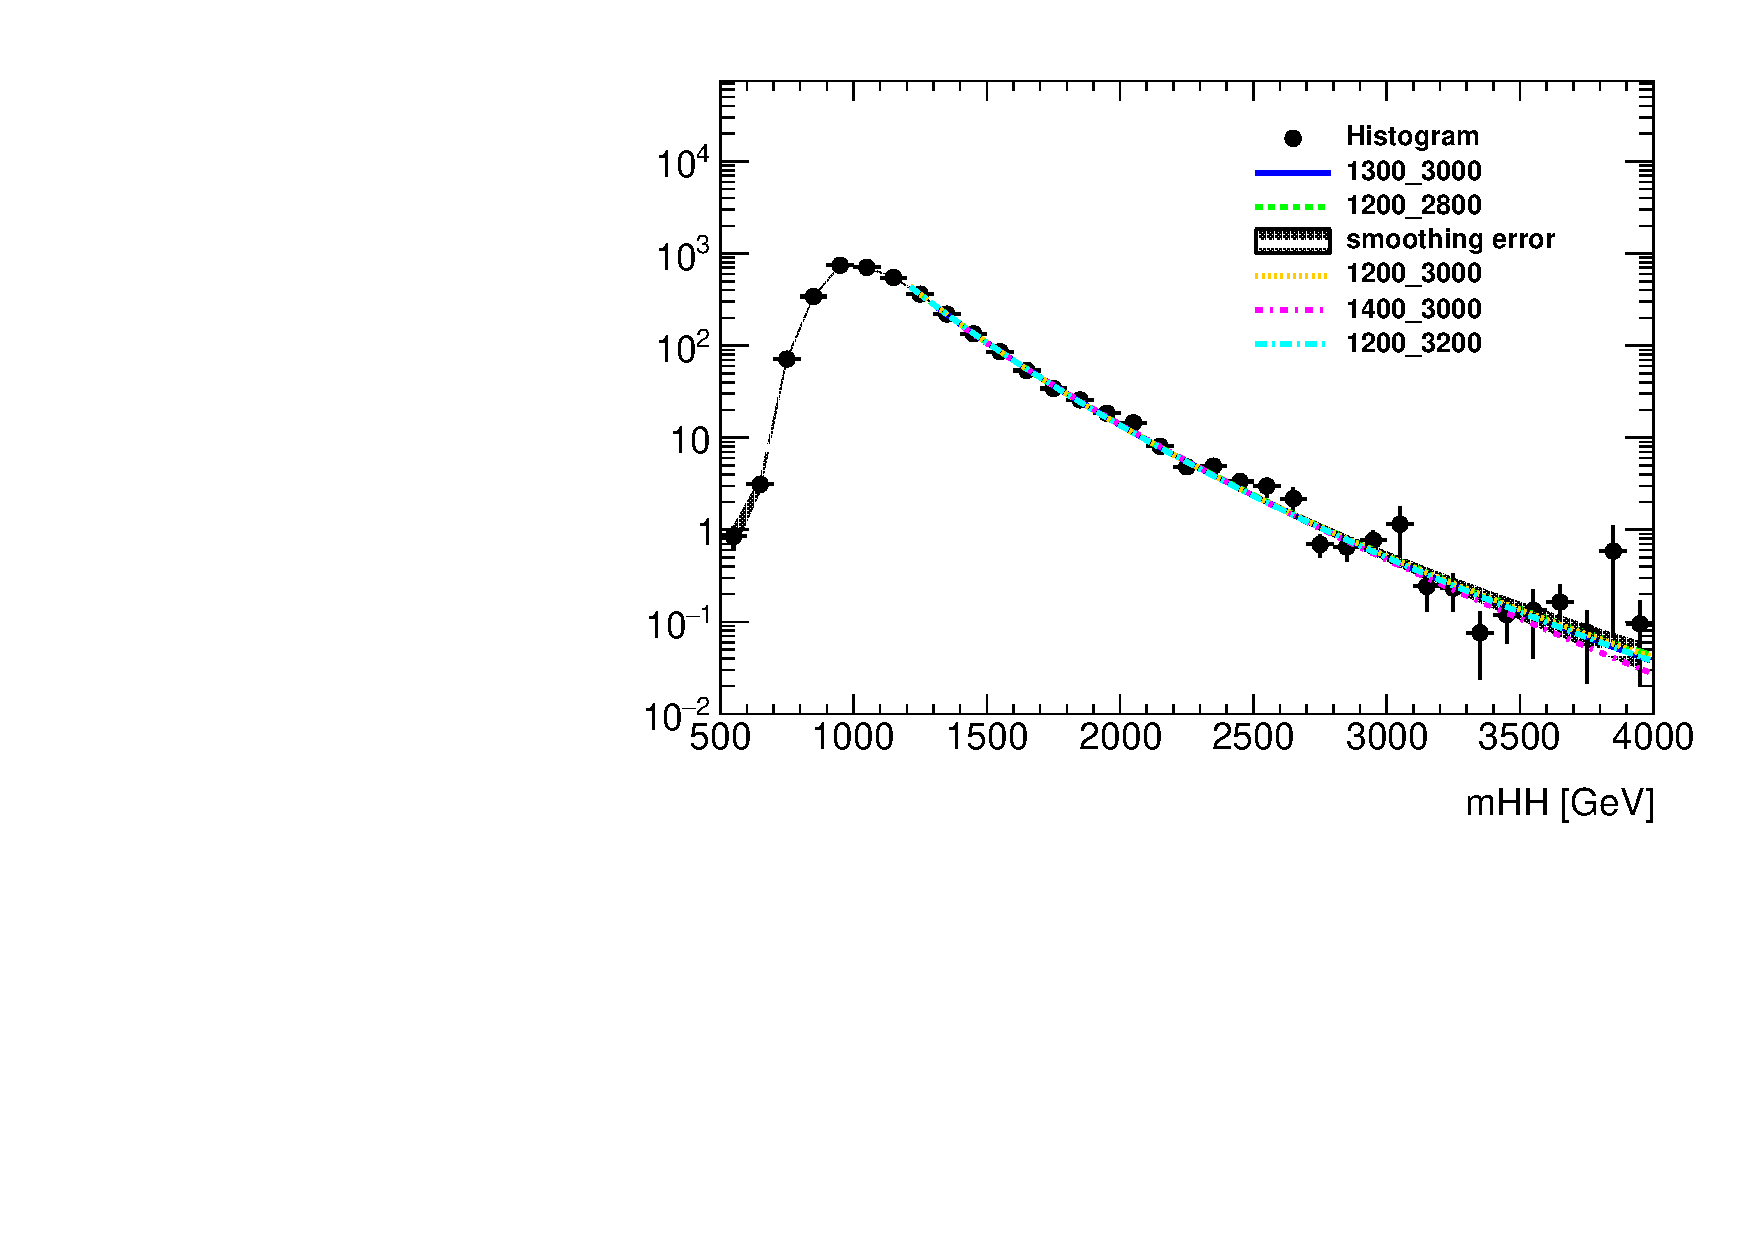
\includegraphics[width=0.31\textwidth,angle=-90]{figures/boosted/Syst_Smooth/smoothFuncRangeCompare_22_comp.pdf}
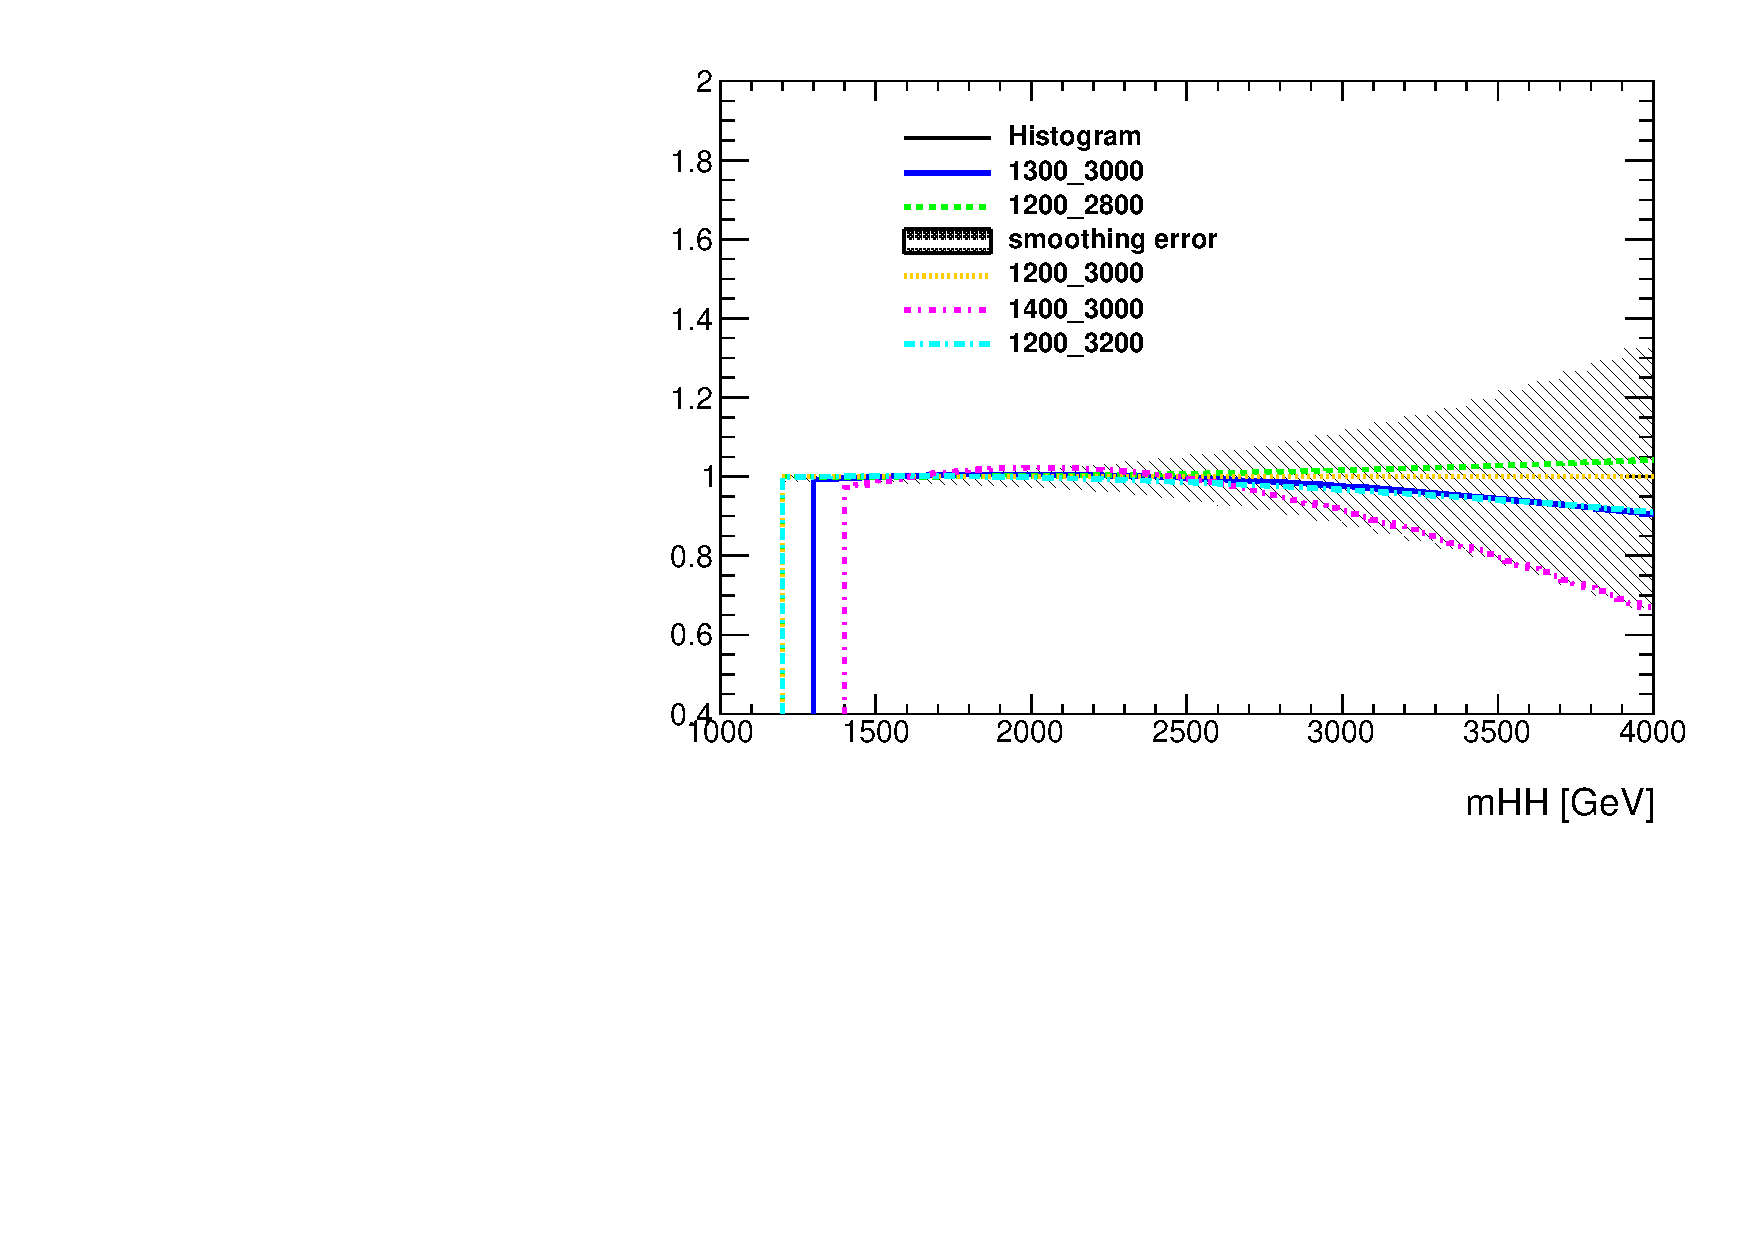
\includegraphics[width=0.31\textwidth,angle=-90]{figures/boosted/Syst_Smooth/smoothFuncRangeCompare_22_comp_ratio.pdf} \\
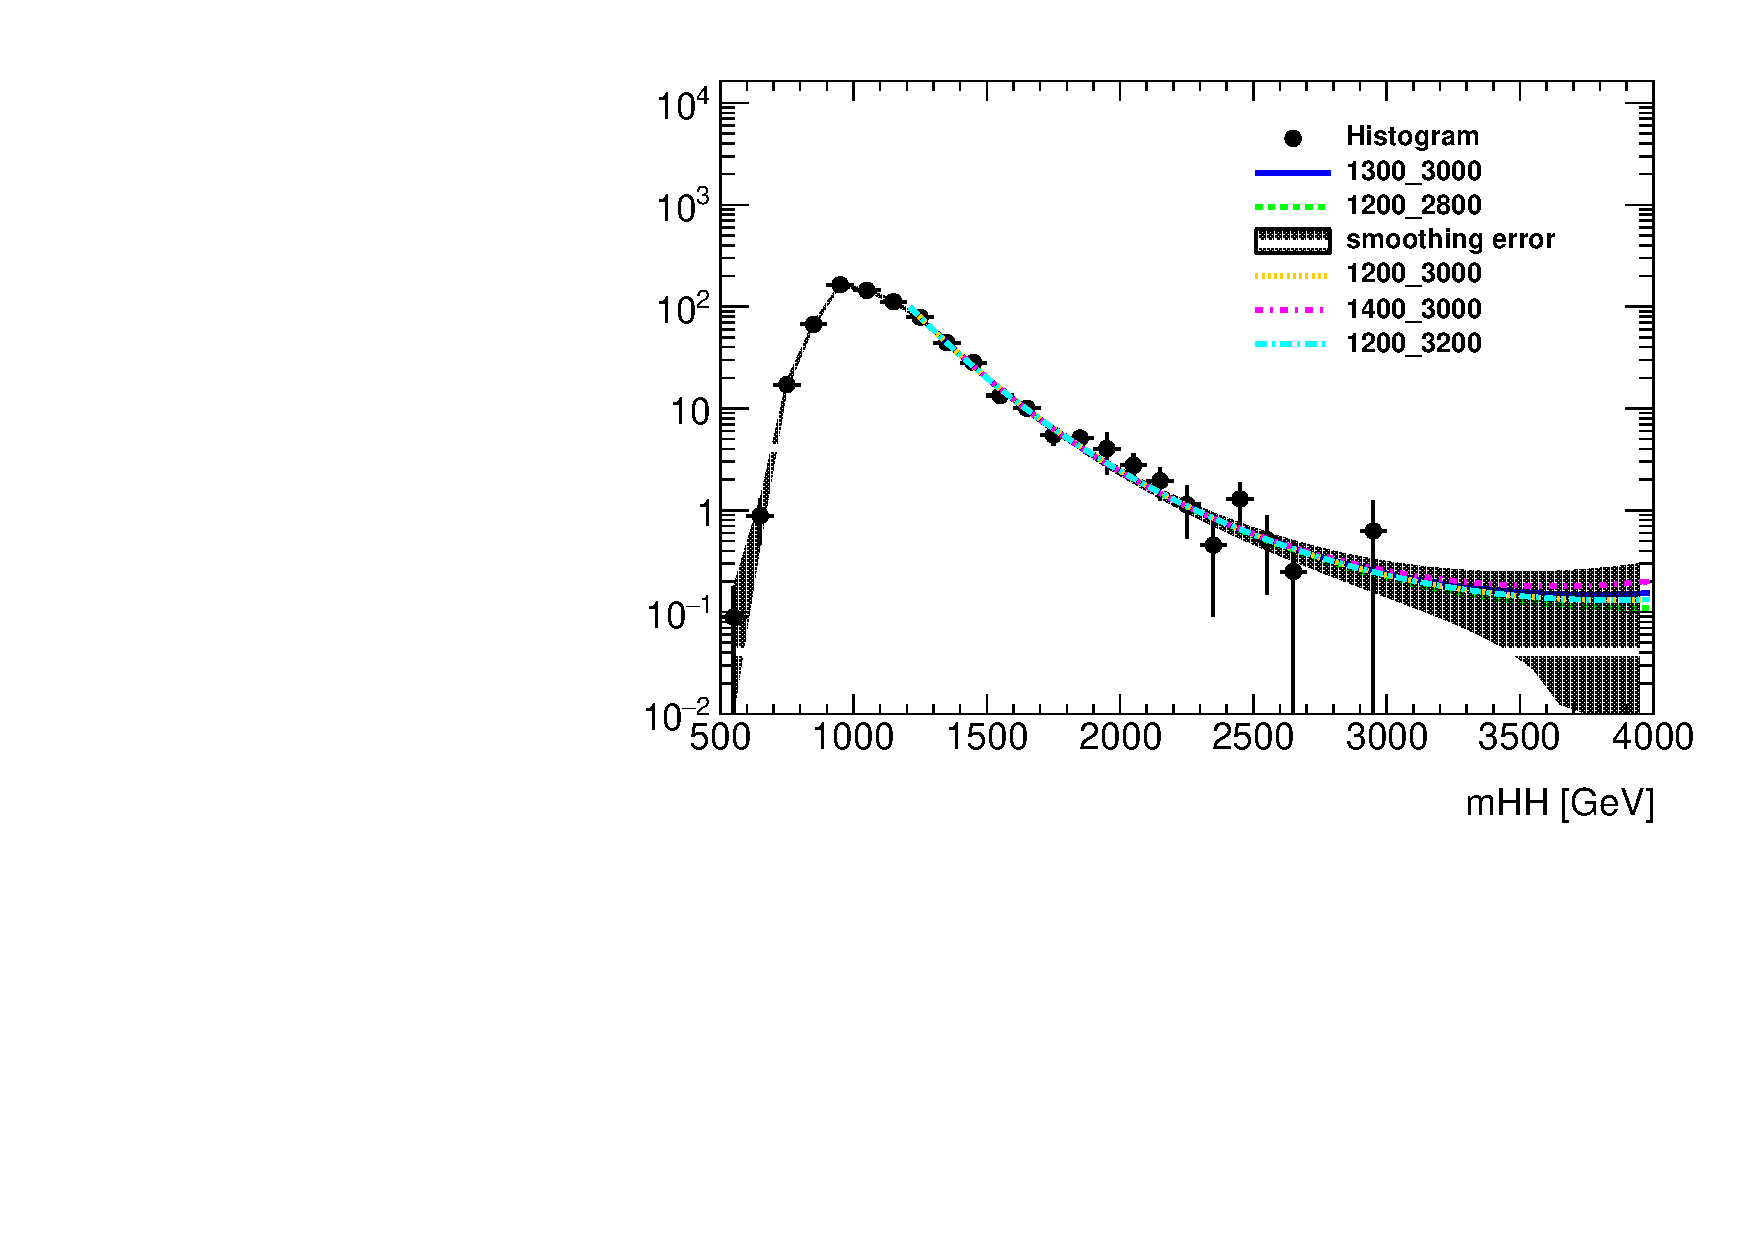
\includegraphics[width=0.31\textwidth,angle=-90]{figures/boosted/Syst_Smooth/smoothFuncRangeCompare_33_comp.pdf}
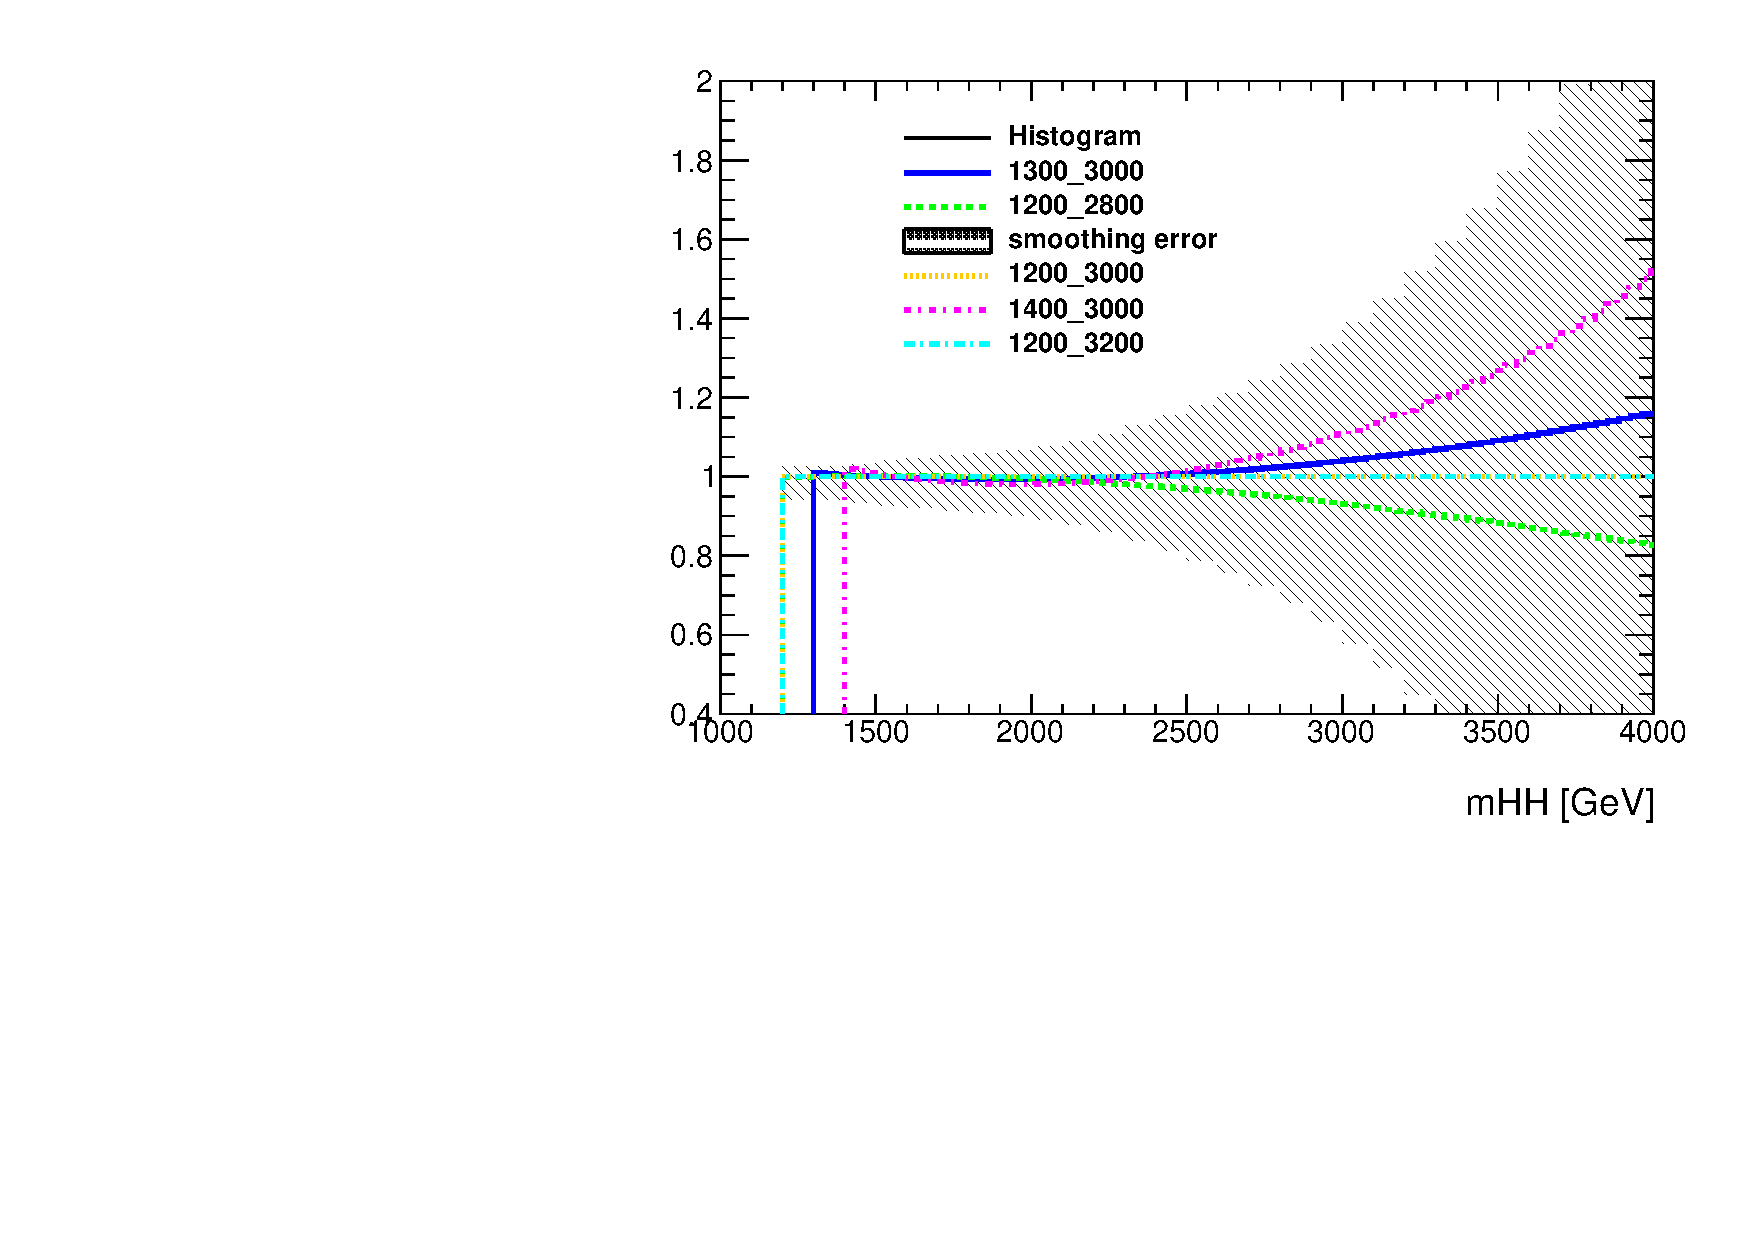
\includegraphics[width=0.31\textwidth,angle=-90]{figures/boosted/Syst_Smooth/smoothFuncRangeCompare_33_comp_ratio.pdf} \\
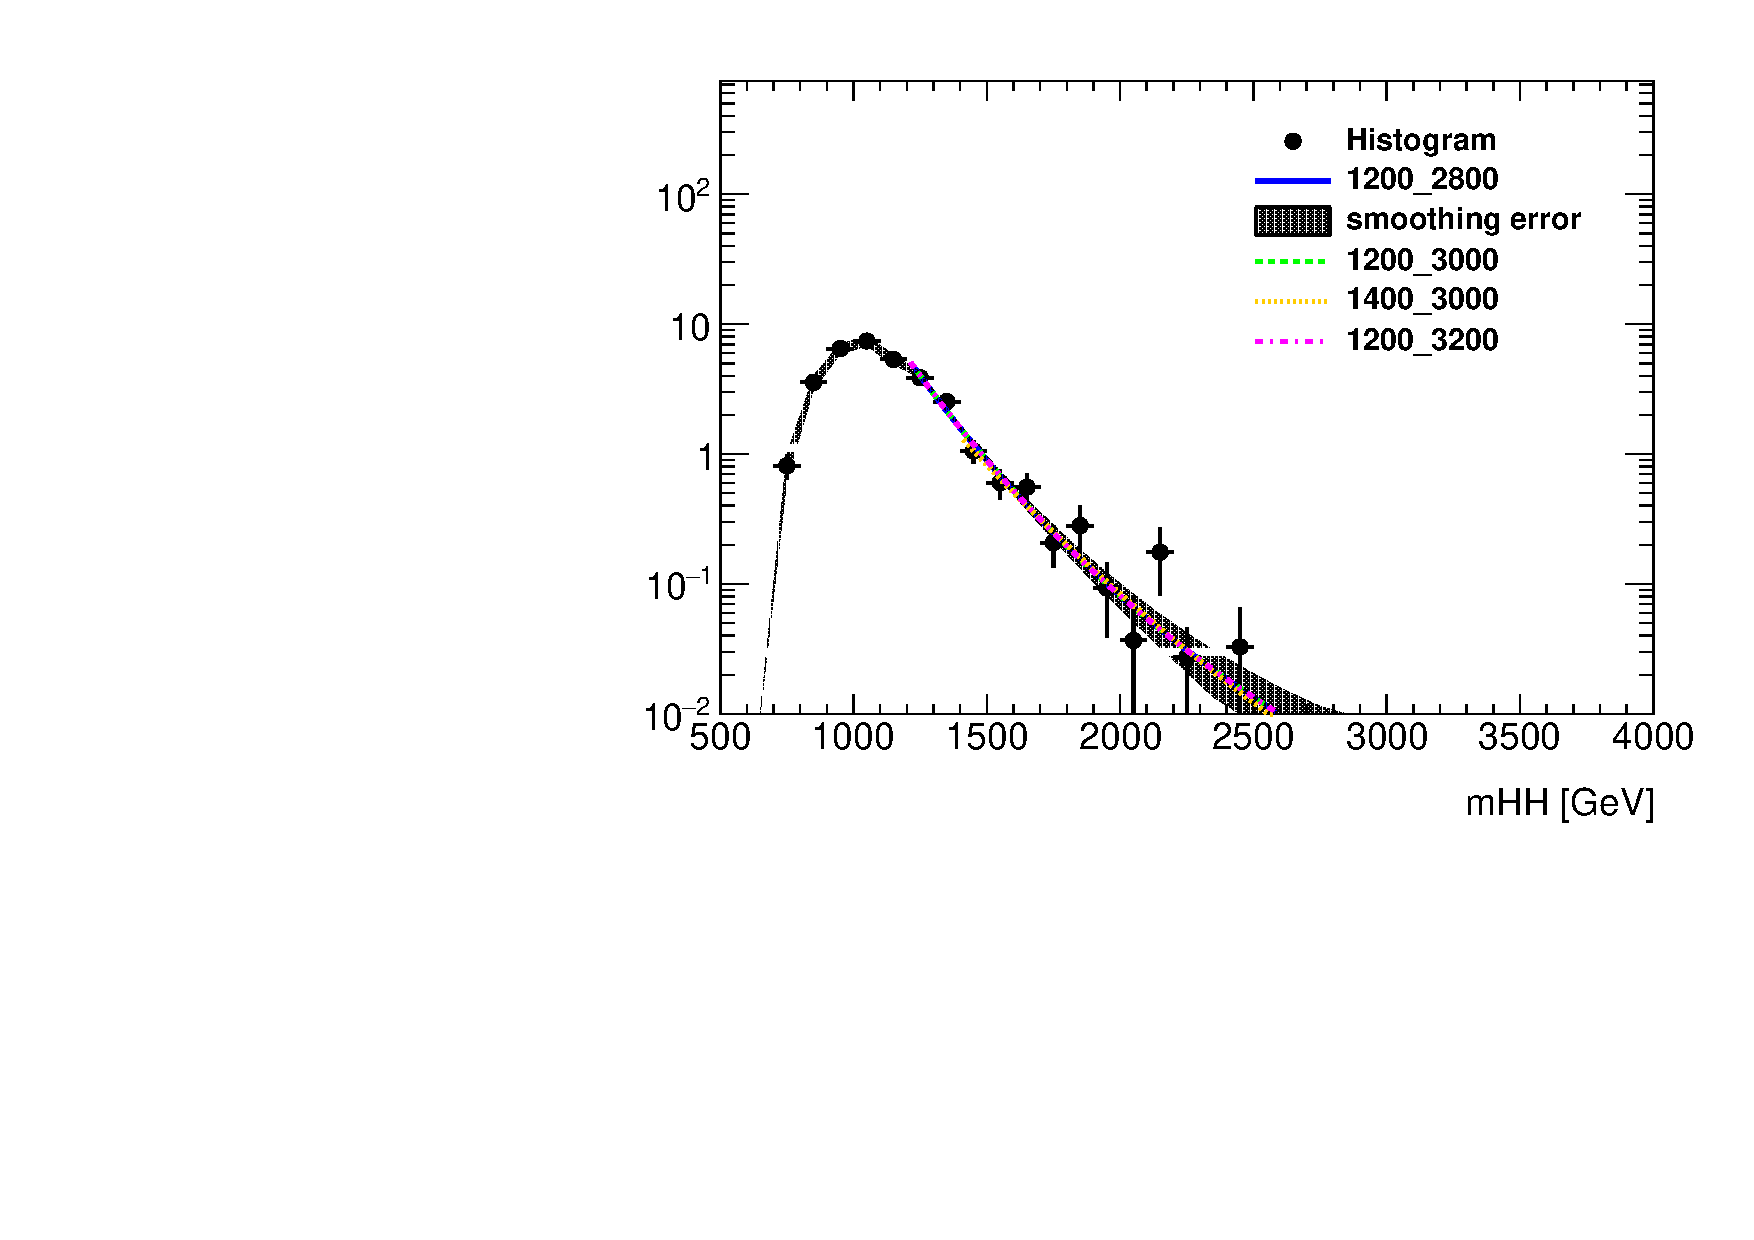
\includegraphics[width=0.31\textwidth,angle=-90]{figures/boosted/Syst_Smooth/smoothFuncRangeCompare_44_comp.pdf}
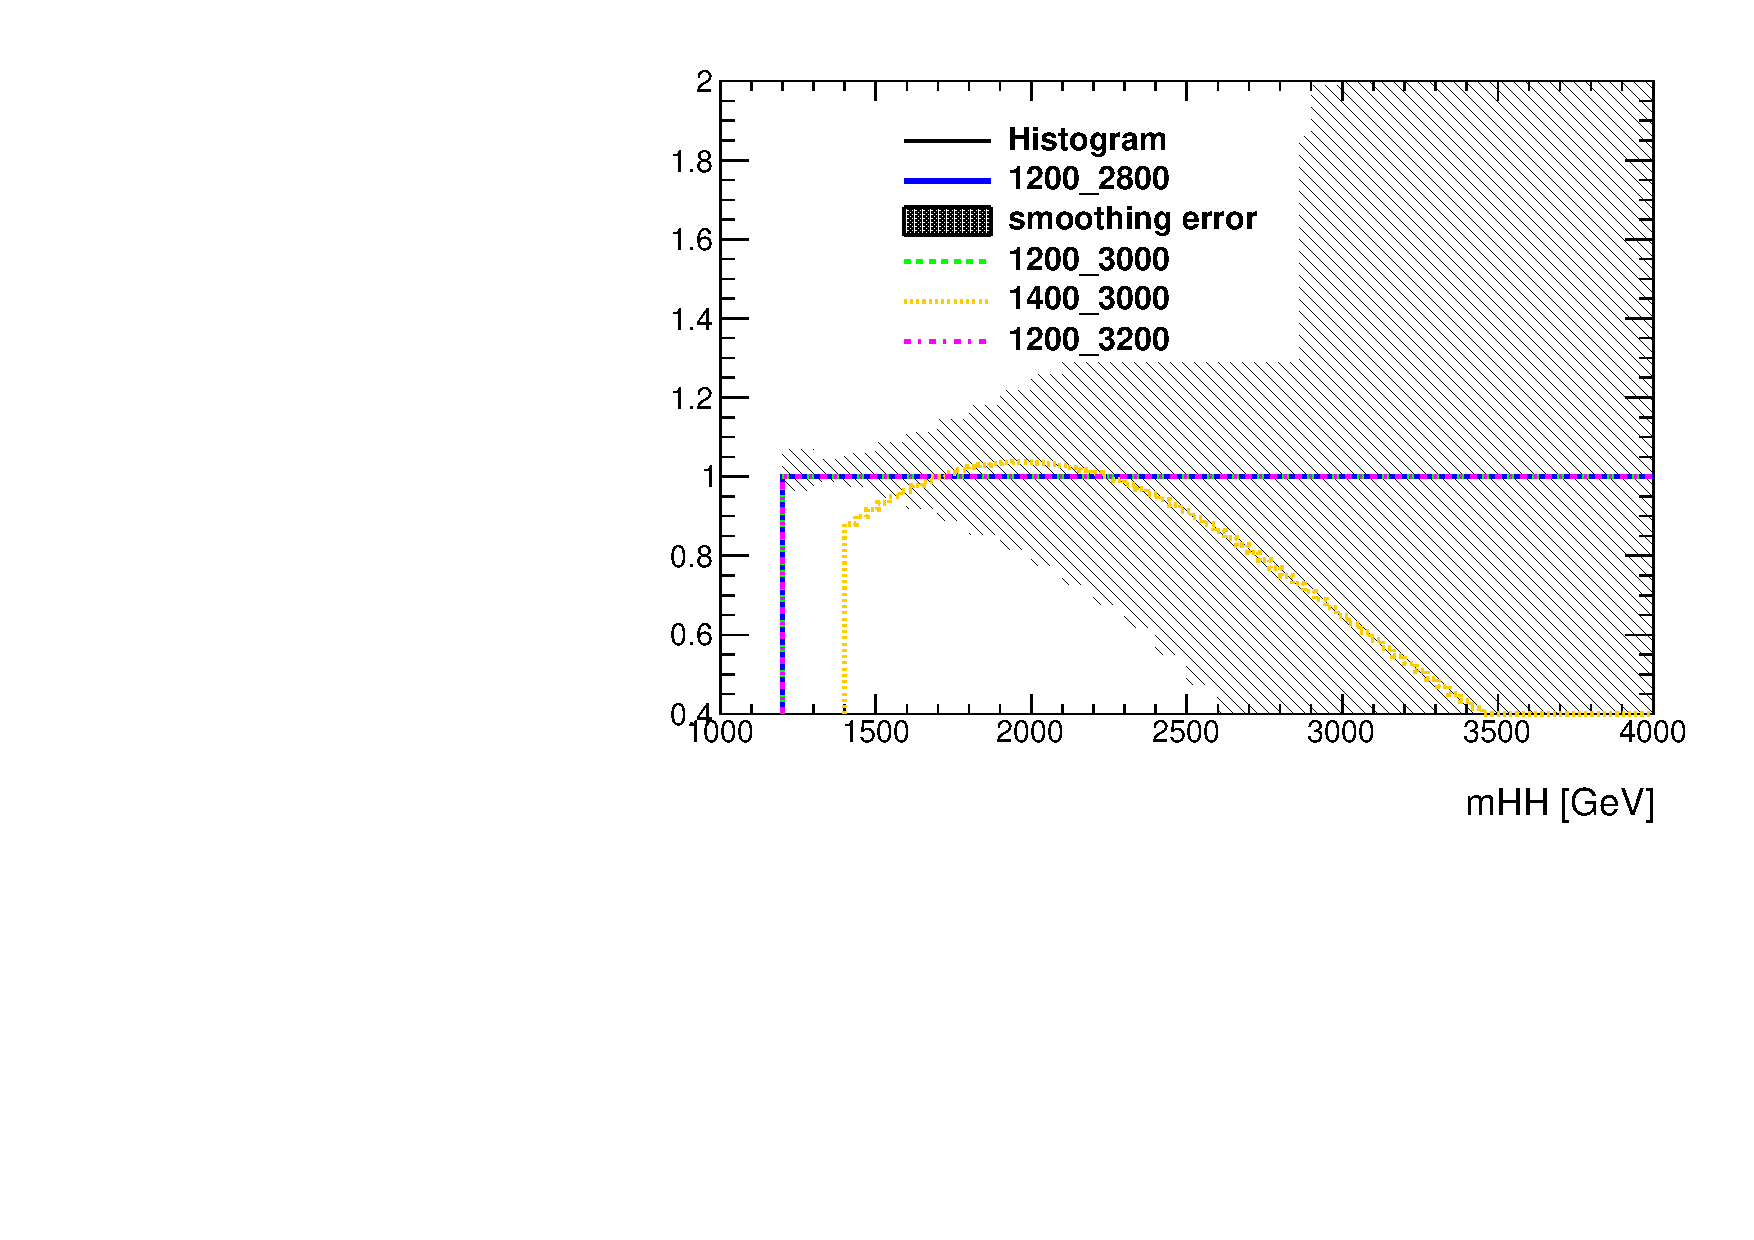
\includegraphics[width=0.31\textwidth,angle=-90]{figures/boosted/Syst_Smooth/smoothFuncRangeCompare_44_comp_ratio.pdf} \\
\caption{Dijet mass distribution SR prediction fit with several fit ranges (left) and the ratio of nominal to fits with different fit ranges (right)  for the $2bs$ (top) $3b$ (middle) and $4b$ (bottom) samples.}
\label{fig:qcd_fit_range_sys_ratio-scaled}
\end{center}
\end{figure}

\paragraph{}
The signal region QCD prediction is also fit with a variety of distributions which have power law behavior in the bulk of the distribution. 
The set of additional functions examined (labeled MJ1-MJ7) can be found in Table~\ref{tab:fit_funcs}, where $x = m_{JJ} / \sqrt{s}$.

\begin{table}[htb!]
\begin{center} 
\begin{tabular}{  l | c}
Name & Functional Form \\
\hline
MJ1 (Dijet) & $f_{1}(x) = p_0 (1-x)^{p_1} x^{p_2}$ \\
MJ2 & $f_{2}(x) = p_0 (1-x)^{p_1} e^{p_2\ x^2}$ \\
MJ3 & $f_{3}(x) = p_0 (1-x)^{p_1} x^{p_2\ x}$ \\
MJ4 & $f_{4}(x) = p_0 (1-x)^{p_1} x^{p_2\ ln\ x}$ \\
MJ5 & $f_{5}(x) = p_0 (1-x)^{p_1} (1+x)^{p_2\ x}$ \\
MJ6 & $f_{6}(x) = p_0 (1-x)^{p_1} (1+x)^{p_2\ ln\ x}$ \\
MJ7 & $f_{7}(x) = \frac{p_0}{x} (1-x)^{p_1 - p_2\ ln\ x}$ \\
MJ8 & $f_{8}(x) = \frac{p_0}{x^2} (1-x)^{p_1 - p_2\ ln\ x}$ \\
\hline
\end{tabular}
\caption{Functions used to fit the QCD dijet mass distributions, where $x = m_{JJ} / \sqrt{s}$.}
\label{tab:fit_funcs}
\end{center}
\end{table}

\paragraph{}
Figure~\ref{fig:qcd_fit_funcs_sys} shows the fits to the QCD prediction in the $4b/3b/2bs$ signal regions, and the nominal dijet fit, as well as the ratios of the nominal fit to that of the additional functions.
As before, poor fits are not used to estimate the uncertainty.

\begin{figure}[htb!]
\begin{center}
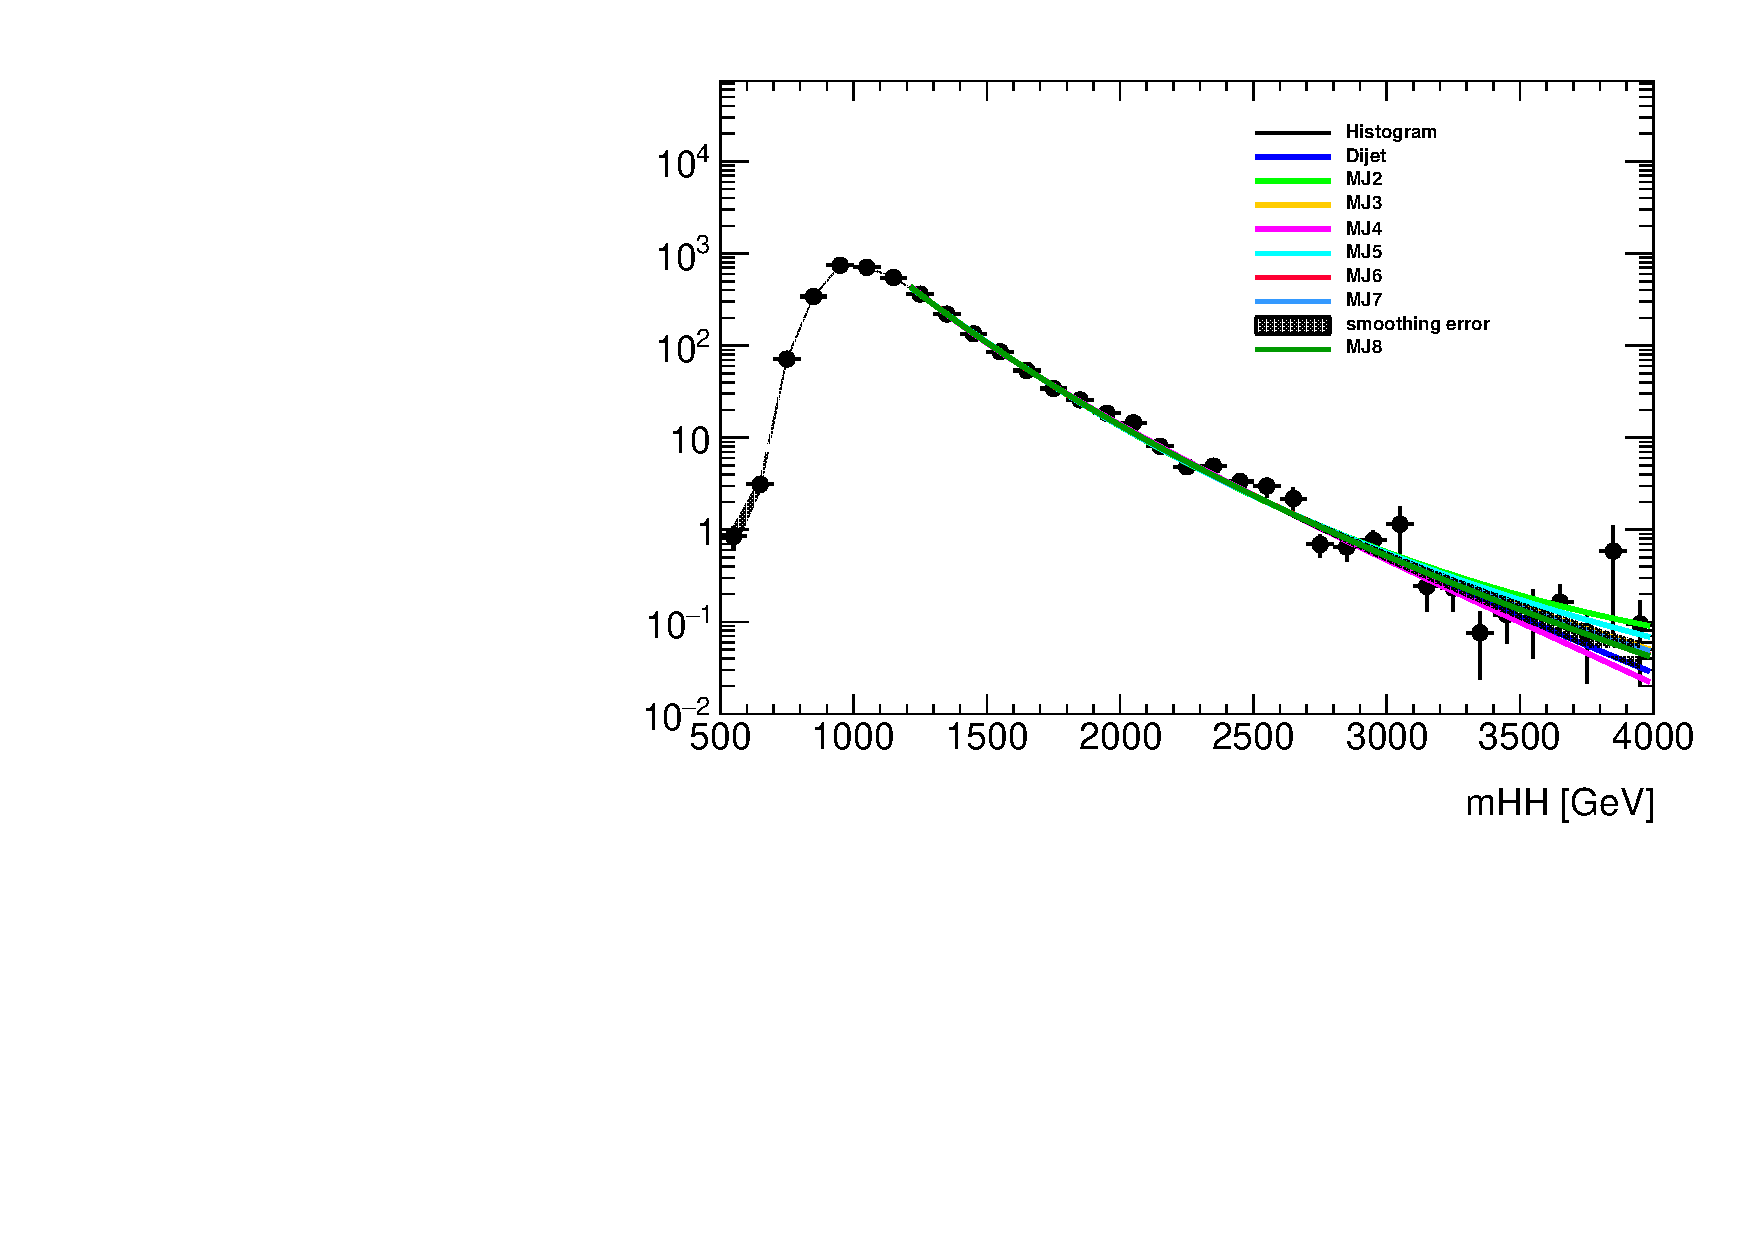
\includegraphics[width=0.31\textwidth,angle=-90]{figures/boosted/Syst_Smooth/smoothFuncCompare_22_comp.pdf}
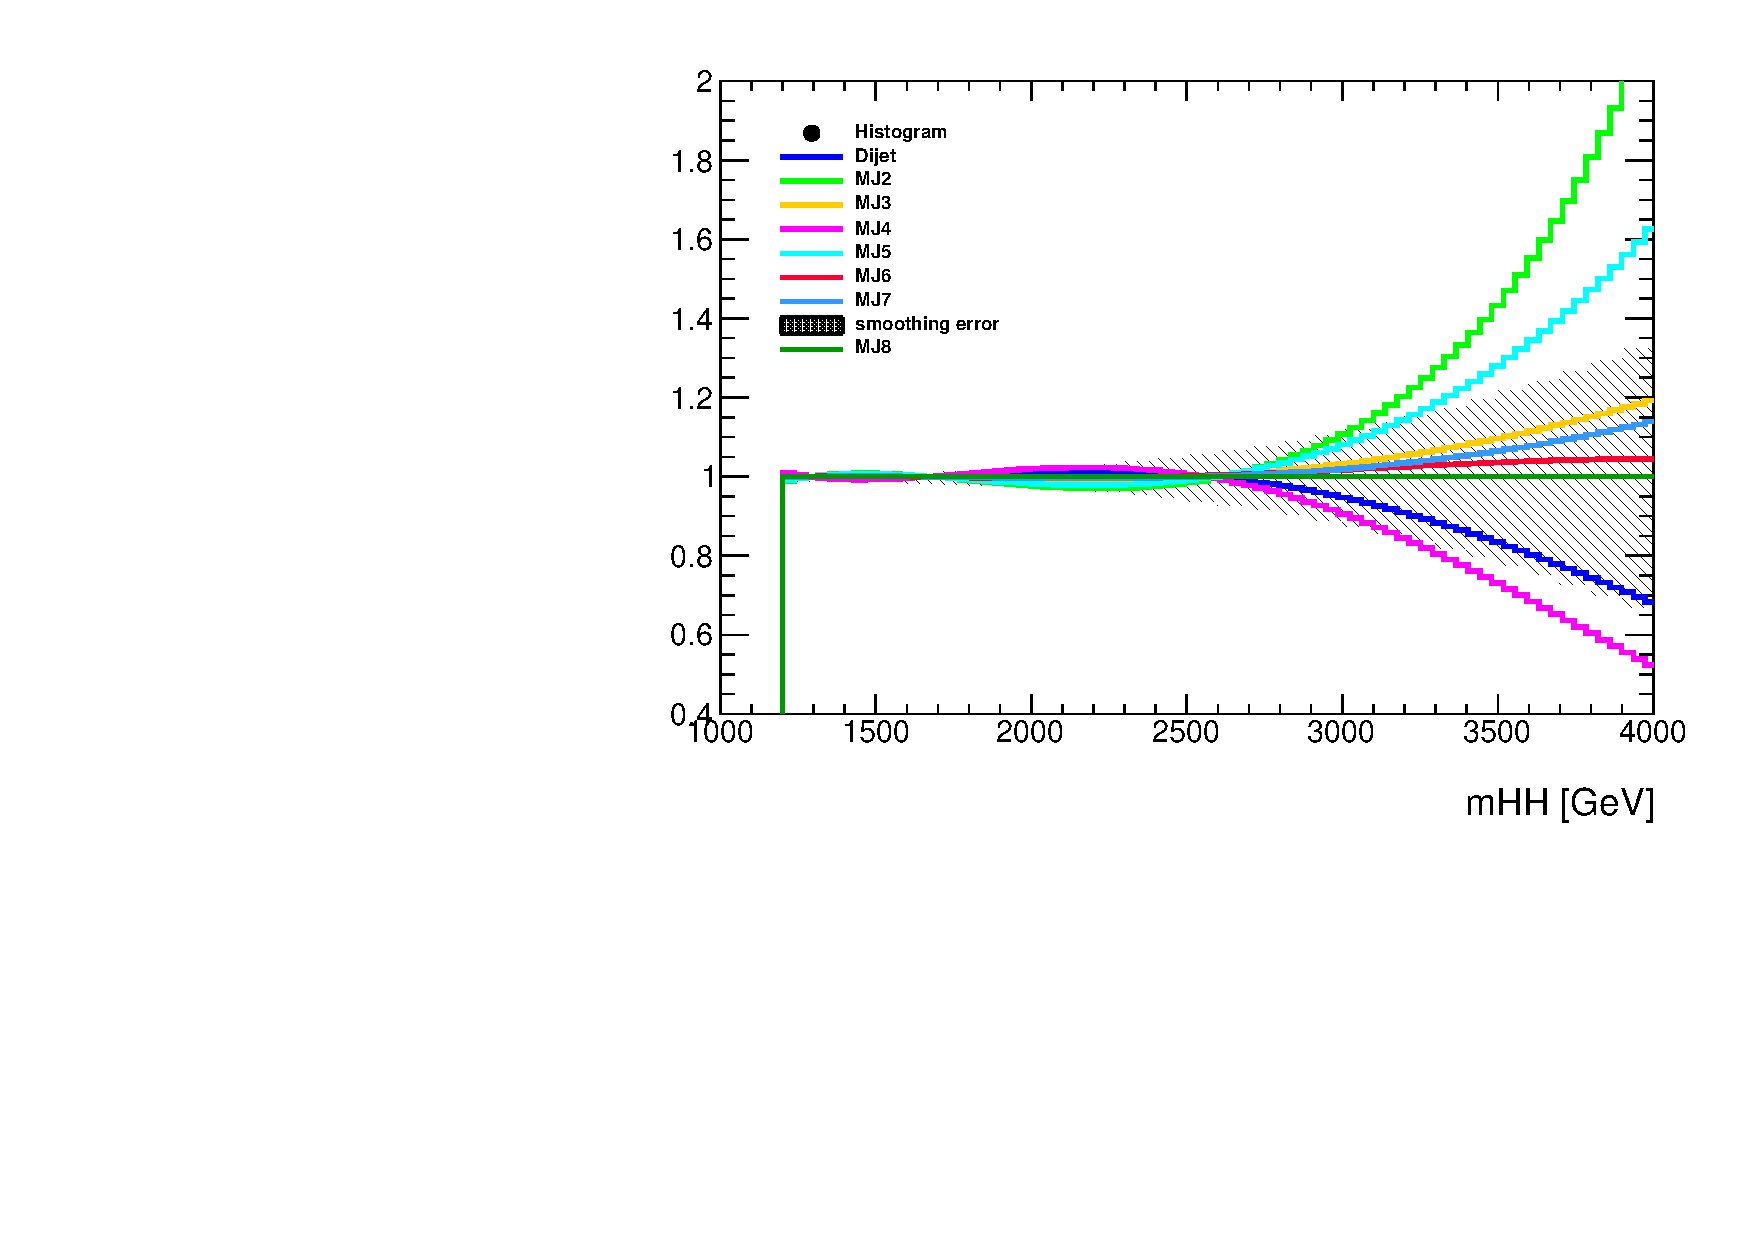
\includegraphics[width=0.31\textwidth,angle=-90]{figures/boosted/Syst_Smooth/smoothFuncCompare_22_comp_ratio.pdf} \\
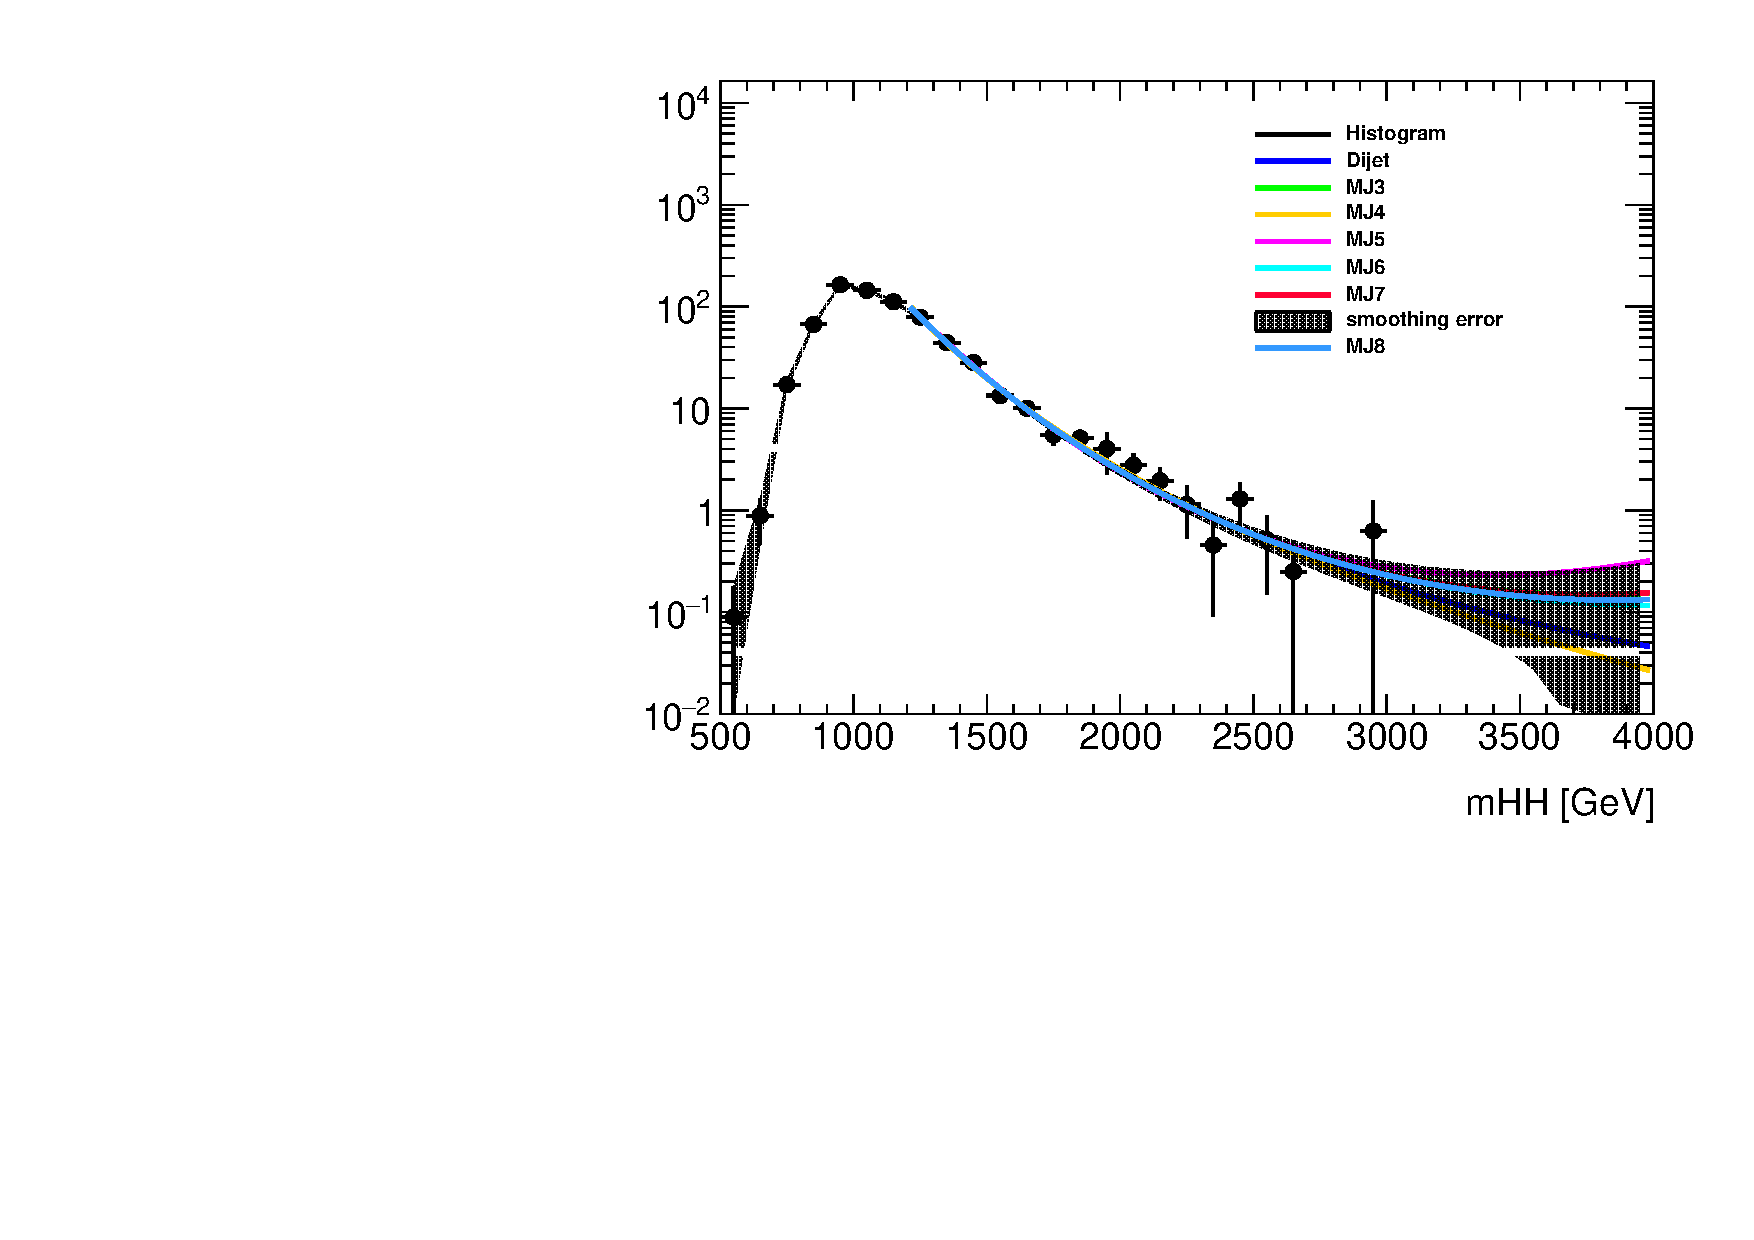
\includegraphics[width=0.31\textwidth,angle=-90]{figures/boosted/Syst_Smooth/smoothFuncCompare_33_comp.pdf}
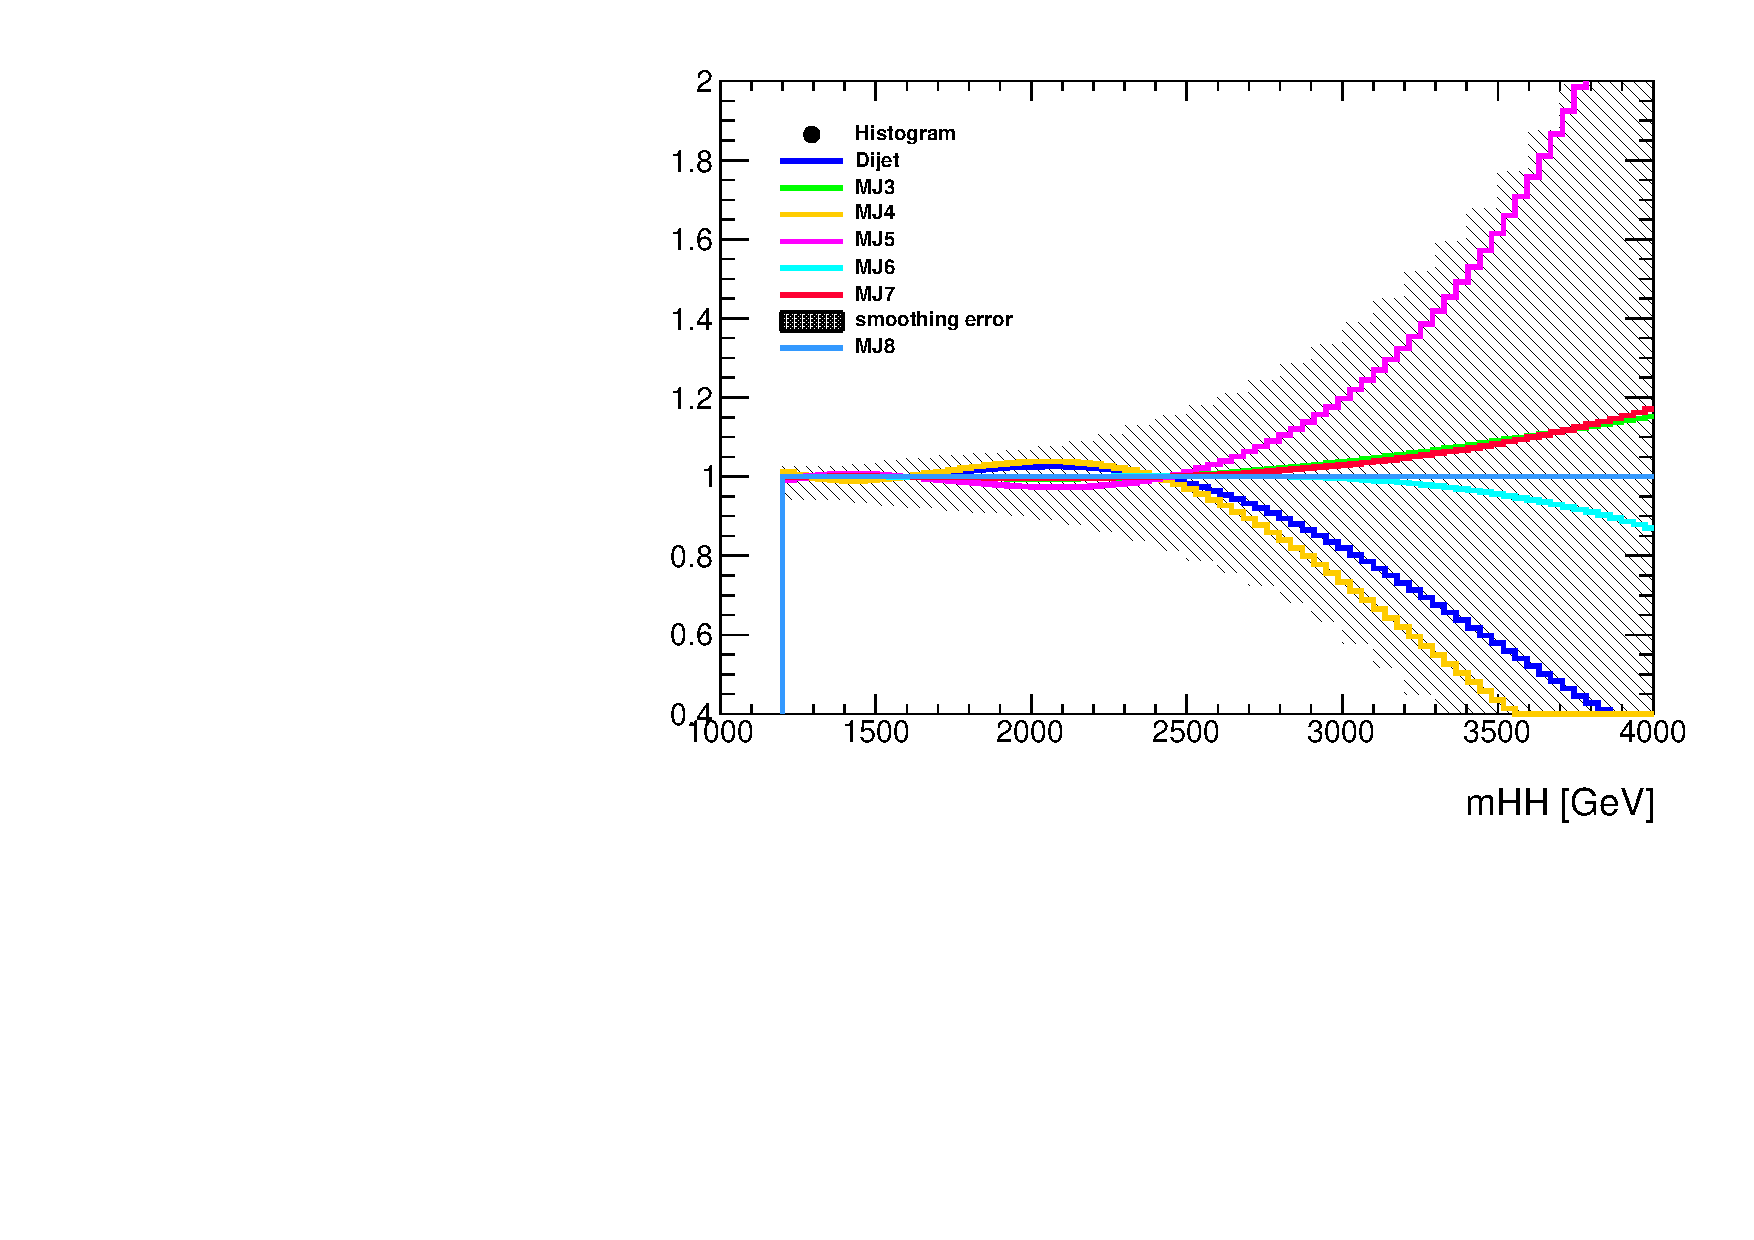
\includegraphics[width=0.31\textwidth,angle=-90]{figures/boosted/Syst_Smooth/smoothFuncCompare_33_comp_ratio.pdf} \\
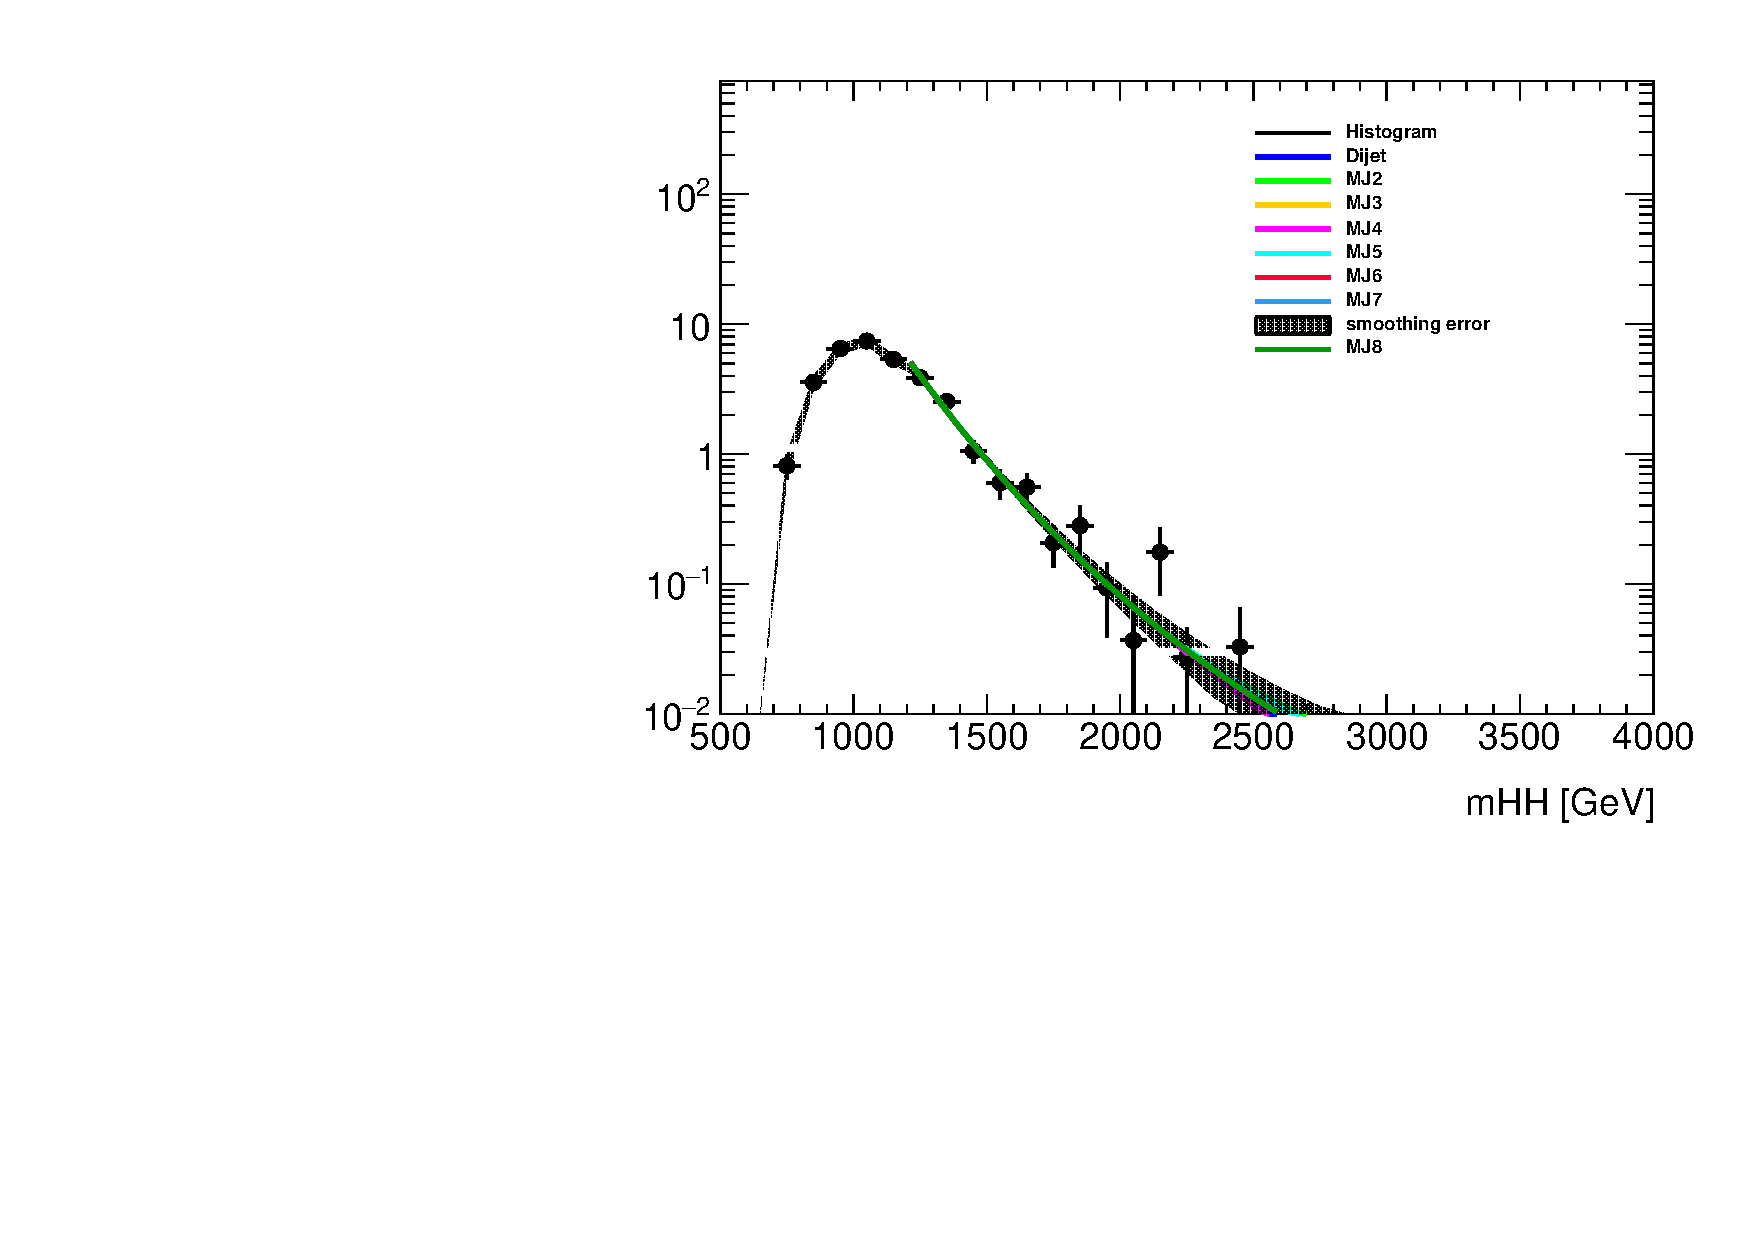
\includegraphics[width=0.31\textwidth,angle=-90]{figures/boosted/Syst_Smooth/smoothFuncCompare_44_comp.pdf}
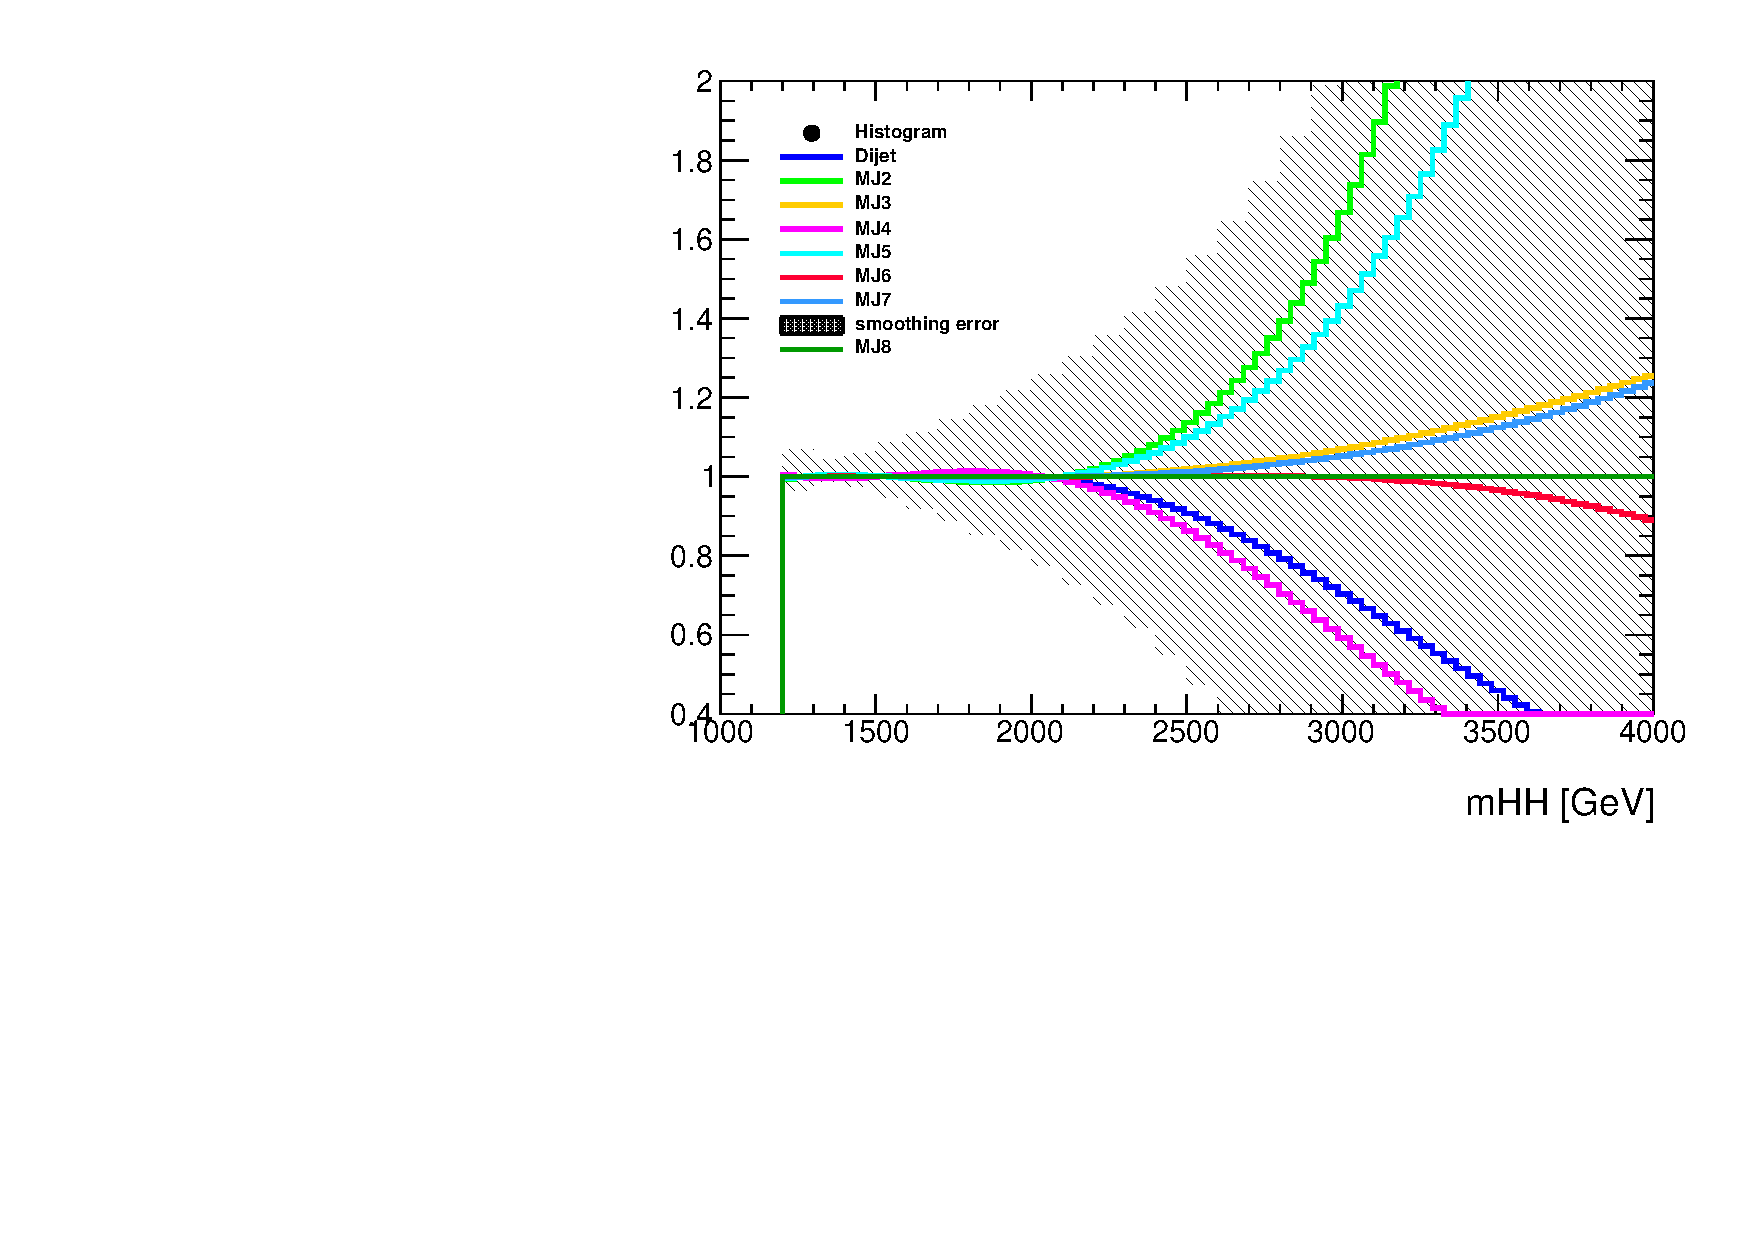
\includegraphics[width=0.31\textwidth,angle=-90]{figures/boosted/Syst_Smooth/smoothFuncCompare_44_comp_ratio.pdf} \\
\caption{ Dijet mass distribution SR prediction fit with several fit functions (left) and the ratio between the nominal function fit result and the fit results with different fit functions (right)  for the $2bs$ (top) $3b$ (middle) and $4b$ (bottom) samples. The additional fit functions are from Table~\ref{tab:fit_funcs}.}
\label{fig:qcd_fit_funcs_sys}
\end{center}
\end{figure}